%% Submissions for peer-review must enable line-numbering
%% using the lineno option in the \documentclass command.
%%
%% Preprints and camera-ready submissions do not need
%% line numbers, and should have this option removed.
%%
%% Please note that the line numbering option requires
%% version 1.1 or newer of the wlpeerj.cls file, and
%% the corresponding author info requires v1.2

\documentclass[fleqn,10pt,lineno]{wlpeerj} % for journal submissions
% \documentclass[fleqn,10pt]{wlpeerj} % for preprint submissions

\newcommand{\cheng}[1]{\textcolor{orange}{\textbf{Cheng: }{\footnotesize #1}}}
\newcommand{\alasdair}[1]{\textcolor{blue}{\textbf{Alasdair: }{\footnotesize #1}}}

\usepackage{bm} % bold math symbols
\usepackage{hyperref} % create hyperlinks
\usepackage[labelfont=bf]{caption} % figure captions
\usepackage{subcaption}
\usepackage[boxed]{algorithm2e} % provide environment and layout to write pseudo-code
\usepackage{IEEEtrantools} % more flexible formatting of equations
\usepackage{mathtools} % use DeclarePairedDelimiterXPP
\usepackage{etoolbox}
\usepackage{tikz} % draw diagrams
\usetikzlibrary{shapes,arrows}
\hypersetup{
	colorlinks   = true, % Colours links instead of ugly boxes
	citecolor    = {blue},
	pdfauthor    = {Alasdair Tran and Cheng Soon Ong},
	pdftitle	 = {Combining Active Learning Suggestions},
}

\DeclareMathAlphabet{\mathcal}{OMS}{cmsy}{m}{n} % reset calligraphy font

% some convenient symbols
\DeclareMathOperator{\Beta}{Beta}
\DeclareMathOperator{\Bin}{Bin}
\DeclareMathOperator{\tr}{tr}
\newcommand{\A}{\mathpzc{A}}
\newcommand{\B}{\mathcal{B}}
\newcommand{\X}{\mathcal{X}}
\newcommand{\Y}{\mathcal{Y}}
\newcommand{\Ecal}{\mathcal{E}}
\newcommand{\Normal}{\mathcal{N}}
\newcommand{\Unlabeled}{\mathcal{U}}
\newcommand{\Labeled}{\mathcal{L}}
\newcommand{\R}{\mathcal{R}}
\newcommand*{\argmin}{\operatornamewithlimits{arg\,min}\limits}
\newcommand*{\argmax}{\operatornamewithlimits{arg\,max}\limits}
\newcommand{\MPBA}{\text{MPBA}}
\newcommand{\passive}{\text{passive}}
\newcommand{\Select}{\textsc{Select}}
\newcommand{\Update}{\textsc{Update}}
\newcommand{\bmu}{\bm{\mu}}
\newcommand{\bsigma}{\bm{\sigma}}
\newcommand{\btau}{\bm{\tau}}

% Expected value
\providecommand\given{}
\DeclarePairedDelimiterXPP\E[1]{\mathbb{E}}{[}{]}{}{
	\renewcommand\given{  \nonscript\:
		\delimsize\vert
		\nonscript\:
		\mathopen{}
		\allowbreak}
	#1
}
% Probability
\DeclarePairedDelimiterXPP\Prob[1]{\mathbb{P}}{(}{)}{}{
	\renewcommand\given{  \nonscript\:
		\delimsize\vert
		\nonscript\:
		\mathopen{}
		\allowbreak}
	#1
}

% Settings for algorithm blocks
\DontPrintSemicolon % don't display semicolons at the end of each line
\SetArgSty{textnormal} % no need to italicise
\SetKwProg{Fn}{function}{}{} % function keyword

% Number paragraphs that are followed by an equation with lineno properly
\newcommand*\patchAmsMathEnvironmentForLineno[1]{%
\expandafter\let\csname old#1\expandafter\endcsname\csname #1\endcsname
\expandafter\let\csname oldend#1\expandafter\endcsname\csname end#1\endcsname
\renewenvironment{#1}%
   {\linenomath\csname old#1\endcsname}%
   {\csname oldend#1\endcsname\endlinenomath}}%
\newcommand*\patchBothAmsMathEnvironmentsForLineno[1]{%
\patchAmsMathEnvironmentForLineno{#1}%
\patchAmsMathEnvironmentForLineno{#1*}}%
\AtBeginDocument{%
\patchBothAmsMathEnvironmentsForLineno{equation}%
\patchBothAmsMathEnvironmentsForLineno{align}%
\patchBothAmsMathEnvironmentsForLineno{IEEEeqnarray}%
}

\title{Combining Active Learning Suggestions}

\author[1, 2]{Alasdair Tran}
\author[1, 3]{Cheng Soon Ong}
\author[4, 5]{Christian Wolf}
\affil[1]{Research School of Computer Science, Australian National University}
\affil[2]{Data to Decisions Cooperative Research Centre, Australia}
\affil[3]{Machine Learning Research Group, Data61, CSIRO, Australia}
\affil[4]{Research School of Astronomy and Astrophysics, Australian National
          University}
\affil[5]{ARC Centre of Excellence for All-sky Astrophysics (CAASTRO)}

\corrauthor[1]{Alasdair Tran}{alasdair.tran@anu.edu.au}

% \keywords{machine learning, active learning, bandit, rank aggregation,
%           expert advice, astronomy}

\begin{abstract}
We study the problem of combining active learning suggestions to identify
informative training examples by empirically comparing methods on benchmark
datasets. Many active learning heuristics for classification problems have been
proposed to help us pick which instance to annotate next. But what is the
optimal heuristic for a particular source of data? Motivated by the success of
methods that combine predictors, we combine active learners with bandit
algorithms and rank aggregation methods. We demonstrate that a combination of
active learners outperforms passive learning in large benchmark datasets and
removes the need to pick a particular active learner a priori. We discuss
challenges to finding good rewards for bandit approaches and show that rank
aggregation performs well.

\end{abstract}

\begin{document}

\flushbottom
\maketitle
\thispagestyle{empty}

\section{Introduction}
Recent advances in sensors and scientific instruments have led to an increasing
use of machine learning techniques to manage the data deluge. Supervised
learning has become a widely used paradigm in many big data applications. This
relies on building a training set of labeled examples, which is time-consuming
as it requires manual annotation from human experts.

In this paper we consider the binary and multiclass classification setting,
where we would like to learn a classifier $h$, which is a function that maps
some feature space $\X \subseteq \mathbb{R}^d$ to a probability distribution
over a finite label space $\Y$:
\begin{IEEEeqnarray}{lCl}
	h : \X \rightarrow p(\Y)
\end{IEEEeqnarray}
In other words, we require that the classifier produces class probability
estimates for each test example. For instance, in logistic regression with only
two classes, i.e. $\Y = \{0, 1\}$, we can model the probability that an object
with feature vector $\bm{x}$ belongs to the positive class with
\begin{IEEEeqnarray}{lCl}
	h(\bm{x}; \bm{\theta}) &=& \Prob{y=1 \given \bm{x}; \bm{\theta}}
	= \dfrac{1}{1 + e^{-\bm{\theta}^T \bm{x}}}
\end{IEEEeqnarray}
and the training process involves learning the optimal weight vector
$\bm{\theta}$. We can further consider kernel logistic regression, where $\X$
is the feature space corresponding to a given kernel, allowing for non-linear
decision functions.

The most common approach to producing a training set is passive learning, where
we randomly select an instance from a large pool of unlabeled data to annotate,
and we continue doing this until the training set reaches a certain size or
until the classifier makes sufficiently good predictions. Depending on how the
underlying data is distributed, this process can be quite inefficient. It seems
that we could exploit the current set of labeled data to identify more
informative unlabeled examples to annotate. For instance, we can pick examples
near the decision boundary of the classifier, where we are still unsure which
class the example belongs to (i.e. where the class probability estimates are
still uncertain).

This led to the development of many active learning heuristics that try to
reduce the labeling bottleneck without sacrificing the classifier performance.
This is done by actively choosing the most informative examples to be labeled
based on the predicted class probabilities. Section~\ref{sec:heuristics}
describes two families of algorithms in detail---uncertainty sampling and
version space reduction.

In this paper, we present a survey of how we can combine suggestions from
various active learning heuristics. In supervised learning, combining
predictors is a well-studied problem. Many techniques such as
AdaBoost~\citep{freund96} (which averages predictions from a set of models) and
decision trees~\citep{breiman84} (which select one model for making predictions
in each region of the input space) have been shown to perform better than just
using a single model. Inspired by this success, we propose to combine active
learning suggestions with bandit and social choice theories in
Section~\ref{sec:expert}. The use of bandit algorithms, where we pick only one
heuristic at each time step, has been studied before~\citep{baram04, hsu15}.
However, as far as we know, this is the first time that social choice theory is
used to rank and aggregate suggestions.

To compare the algorithms, we run them on 11 benchmark datasets from the UCI
Machine Learning Repository~\citep{lichman13} and a large dataset from the
Sloan Digital Sky Survey (SDSS)~\citep{alam15}. The experimental setup and
discussion are described in Section~\ref{sec:expt} and~\ref{sec:discuss}.


\section{Overview of Active Learning}~\label{sec:heuristics}
Recall that in active learning, we exploit the class probability estimates from
a trained classifier to estimate a score of informativeness for each test
example. In pool-based active learning, where we select an object from a pool
of unlabeled examples at each time step, we require that some objects have
already been labeled. In practice, this normally means that we label a small
random sample at the beginning. These become the labeled training set
$\Labeled_T \subset \X \times \Y$, and the rest form the unlabeled set
$\Unlabeled \subset \X$.

Now consider the problem of choosing the next example in $\Unlabeled$ for
querying. Labeling can be a very expensive task, because it requires using
expensive equipment or human experts to manually examine each object. Thus we
want to be smart in choosing the next example. This motivates us to come up
with a rule $s(\bm{x}; h)$ that gives each unlabeled example a score based only
on their feature vector $\bm{x}$ and the current classifier $h$. Recall that
the classifier produces $p(\Y)$, a probability estimate for each class. We can
use these probability estimates to calculate the scores:
\begin{IEEEeqnarray}{lCl}
	s : p(\Y) \rightarrow \mathbb{R}
\end{IEEEeqnarray}
The value of $s(\bm{x}; h)$ indicates the informativeness of example $\bm{x}$,
where bigger is better. Thus we would like to choose the example with the
largest value of $s(\bm{x}; h)$. This will be our active learning rule $r$:
\begin{IEEEeqnarray}{lCl}
	r(\bm{x}; h) &=& \argmax_{\bm{x} \in \Unlabeled} s(\bm{x}; h)
\end{IEEEeqnarray}
Algorithm~\ref{alg:active} outlines the standard pool-based active learning
setting.

\begin{algorithm}[htbp]
	\KwIn{
    	unlabeled set $\Unlabeled$,
        labeled training set $\Labeled_T$,
        classifier $h(\bm{x})$,
        and active learner $r(\bm{x}; h)$.
        }
    \BlankLine
	\Repeat{we have enough training examples.}{
		Select the most informative candidate $\bm{x}_*$ from $\Unlabeled$ using the
			active learning rule $r(\bm{x}; h)$. \;
        Ask the expert to label $\bm{x}_*$. Call the label $y_*$. \;
		Add the newly labeled example to the training set:
			$\Labeled_T \leftarrow \Labeled_T  \cup \{(\bm{x}_*, y_*)\}$. \;
		Remove the newly labeled example from the unlabeled set:
			$\Unlabeled \leftarrow \Unlabeled \setminus \{ \bm{x}_* \}$. \;
        Retrain the classifier $h(\bm{x})$ using $\Labeled_T$. \;
    }

	\caption{The pool-based active learning algorithm.}
	\label{alg:active}
\end{algorithm}

Coming up with an optimal rule is itself a difficult problem, but there have
been many attempts to derive good heuristics. Five common ones, which we shall
use in our experiments, are described in Section~\ref{subsec:uncertainty}
and~\ref{subsec:version}. They roughly fall into two categories: uncertainty
sampling and version space reduction. There are also heuristics that involve
minimizing the variance or maximizing the classifier certainty of the model
\citep{schein07}, but we do not consider them in this paper as they are
computationally inefficient.

\subsection{Uncertainty Sampling}~\label{subsec:uncertainty}
\cite{lewis94} introduced the idea of uncertainty sampling, where we select the
instance whose class membership the classifier is least certain about. These
tend to be points that are near the decision boundary of the classifier.
Perhaps the simplest way to quantify uncertainty is~\cite{culotta05}'s least
confidence heuristic, where we pick the candidate whose most likely label the
classifier is most uncertain about:
\begin{IEEEeqnarray}{lCl}
	r_{LC}(\bm{x}; h) &=& \argmax_{\bm{x} \in \Unlabeled}
	\left\{ - \max_{y \in \Y} p(y | \bm{x}; h) \right\}
\end{IEEEeqnarray}
where $p(y | \bm{x}; h)$ is the probability that the object with feature vector
$\bm{x}$ belongs to class $y$ under classifier $h$. For consistency, we have
flipped the sign of the score function so that the candidate with the highest
score is picked.

A second option is to calculate the entropy \citep{shannon48}, which measures
the amount of information needed to encode a distribution. Intuitively, the
closer the class probabilities of an object are to a uniform distribution, the
higher its entropy will be. This gives us the heuristic of picking the
candidate with the highest entropy of the distribution over the classes:
\begin{IEEEeqnarray}{lCl}
	r_{HE}(\bm{x}; h) &=& \argmax_{\bm{x} \in \Unlabeled}
	\left\{ - \sum_{y \in \Y} p(y | \bm{x}; h)
	\log \big[ p(y | \bm{x}; h) \big] \right\}
\end{IEEEeqnarray}
As a third option we can pick the candidate with the smallest margin, which is defined as
the difference between the two highest class probabilities \citep{scheffer01}:
\begin{IEEEeqnarray}{lCl}
	r_{SM}(\bm{x}; h) &=& \argmax_{\bm{x} \in \Unlabeled}
	\left\{ - \left ( \max_{y \in \Y} p(y | \bm{x}; h) -
	\max_{z \in \Y \setminus \{y^*\}} p(z | \bm{x}; h) \right) \right\}
\end{IEEEeqnarray}
where $y^* = \argmax_{y \in \Y} p(y | \bm{x}; h)$ and we again flip the sign
of the score function. Since the sum of all probabilities must be 1, the
smaller the margin is, the more uncertain we are about the object's class
membership.

\subsection{Version Space Reduction}~\label{subsec:version}
Instead of focusing on the uncertainty of individual predictions, we could
instead try to constrain the size of the version space, thus allowing the
search for the optimal classifier to be more precise. The version space is
defined as the set of all possible classifiers that are consistent with the
current training set. To quantify the size of this space, we can train a
committee of $B$ classifiers, $\B = \{h_1, h_2, ..., h_B\}$, and measure the
disagreement among the members of the committee about an object's class
membership. Ideally, each member should be as different from the others as
possible but still be in the version space \citep{melville04}. In order to have
this diversity, we give each member only a subset of the training examples.
Since there might not be enough training data, we need to use bootstrapping and
select samples with replacement. Hence this method is often called Query by
Bagging (QBB).

One way to measure the level of disagreement is to calculate the margin using
the class probabilities estimated by the committee \citep{melville04}:
\begin{IEEEeqnarray}{lCl}
	r_{QBBM}(\bm{x}; h) &=& \argmax_{\bm{x} \in \Unlabeled}
	\left\{ - \left( \max_{y \in \Y} p(y | \bm{x}; \B) -
	\max_{z \in \Y \setminus \{y^*\}} p(z | \bm{x}; \B) \right) \right\}
\end{IEEEeqnarray}
where
\begin{IEEEeqnarray}{rCl}
	y^* &=& \argmax_{y \in \Y} p(y | \bm{x}; \B) \\
	p(y | \bm{x}; \B) &=& \dfrac{1}{B} \sum_{b \in \B} p(y | \bm{x}; h_b)
\end{IEEEeqnarray}
This looks similar to one of the uncertainty sampling heuristics, except now we
use $p(y | \bm{x}; \B)$ instead of $ p(y | \bm{x}; h)$. That is, we first
average out the class probabilities predicted by the members before minimizing
the margin.~\cite{mccallum98} offered an alternative disagreement measure which
involves picking the candidate with the largest mean Kullback-Leibler (KL)
divergence from the average:
\begin{IEEEeqnarray}{lCl}
	r_{QBBKL}(\bm{x}; h) &=& \argmax_{\bm{x} \in \Unlabeled}
	\left\{ \dfrac{1}{B}
	\sum_{b \in \B} D_{\mathrm{KL}}(p_b\|p_\B) \right\}
\end{IEEEeqnarray}
where $D_{\mathrm{KL}}(p_b\|p_\B)$ is the KL divergence from $p_\B$ (the
probability distribution that is averaged across the committee $\B$), to $p_b$
(the distribution predicted by a member $b \in \B$):
\begin{IEEEeqnarray*}{lCl}
	D_{\mathrm{KL}}(p_b\|p_\B) = \sum_{y \in \Y} p(y | \bm{x}; h_b) \,
								 \ln\frac{p(y | \bm{x}; h_b)}{p(y | \bm{x}; \B)}
\end{IEEEeqnarray*}
For convenience, we summarize the five heuristics discussed above in
Table~\ref{tab:heuristics}.

\begin{table}[tbp]
	\caption {Summary of active learning heuristics used in our experiments.
			  Notations: $p(y | \bm{x}; h)$ is the probability of that an
			  object with feature vector $\bm{x}$ has label $y$ under
			  classifier $h$, $\B$ is the set of $B$ classifiers $\{h_1, h_2,
			  ..., h_B\}$, $\Y$ is the set of possible labels, $y^*$ is the
			  most certain label, $\Unlabeled$ is the set of unlabeled
			  instances, $D_{\mathrm{KL}}(p\|q)$ is the Kullback-Leibler
			  divergence of $p$ from $q$, and $p_\B$ is the class distribution
			  averaged across classifiers in $\B$. For consistency, with
			  heuristics that use minimization, we flip the sign of the score
			  so that we can always take the argmax to get the best candidate.}
	\label{tab:heuristics}
	\centering
	\begin{tabular}{llll}
		\toprule
		Abbreviation & {Heuristic}  &  Objective Function  \\
		\midrule
        \textsc{confidence} & Least Confidence &
			$\argmax_{\bm{x} \in \Unlabeled}
			\left\{ - \max_{y \in \Y} p(y | \bm{x}; h) \right\}$ \\
		\textsc{entropy} & Highest Entropy &
			$\argmax_{\bm{x} \in \Unlabeled} \left\{-\sum_{y \in \Y} p(y | \bm{x}; h)
            \log \big[ p(y | \bm{x}; h) \big] \right\}$
			\\[2ex]
		\textsc{margin} & Smallest Margin &
			$\argmax_{\bm{x} \in \Unlabeled} \left\{ - \left( \max_{y \in \Y} p(y | \bm{x}; h) -
            \max_{z \in \Y \setminus \{y^*\}} p(z | \bm{x}; h) \right) \right\}$
			\\[2ex]
		\textsc{qbb-margin} & Smallest QBB Margin &
			$\argmax_{\bm{x} \in \Unlabeled} \left\{ - \left( \max_{y \in \Y} p(y | \bm{x}; \B) -
            \max_{z \in \Y \setminus \{y^*\}} p(z | \bm{x}; \B) \right) \right\}$
			\\[2ex]
		\textsc{qbb-kl} & Largest QBB KL &
			$\argmax_{\bm{x} \in \Unlabeled} \left\{ \dfrac{1}{B}
               \sum_{b \in \B} D_{\mathrm{KL}}(p_b\|p_\B) \right\}$
			\\
		\bottomrule
	\end{tabular}
\end{table}

\section{Combining Suggestions}~\label{sec:expert}
Out of the five heuristics discussed, how do we know which one is the most
optimal one? There have been some attempts in the literature to do a
theoretical analysis. Proofs are however scarce, and when there is one
available, they normally only work under restrictive assumptions. For example,
\cite{freund97} showed that the query by committee algorithm (a slight variant
of our two QBB heuristics) guarantees an exponential decrease in the prediction
error with the training size, but only when there is no noise. In general,
whether any of these heuristics is guaranteed to beat passive learning is still
an open question.

Even though we do not know which one is the best, we can still combine
suggestions from all of the heuristics. This can be thought of as the problem
of prediction with expert advice, where each expert is an active learning
heuristic. In this paper we explore two different approaches. We can either
consider the advice of only one expert at each time step (with bandit
algorithms), or we can aggregate the advice of all the experts (with social
choice theory).

\subsection{Combining Suggestions with Bandit Theory}\label{subsec:bandit}

First let us turn our attention to the multi-armed bandit problem in
probability theory. The colorful name originates from the situation where a
gambler stands in front of a slot machine with $R$ levers. When pulled, each
lever gives out a reward according to some unknown distribution. The goal of
the game is to come up with a strategy that can maximize the gambler's lifetime
rewards while minimizing the number of pulls. In the context of active
learning, each lever is a heuristic with a different ability to identify the
candidate whose labeling information is most valuable.

The main problem in multi-armed bandits is the trade-off between exploring
random heuristics and exploiting the best heuristic so far. There are many
situations in which we find our previously held beliefs to be completely wrong.
By always exploiting, we could miss out on the optimal heuristic. On the other
hand, if we explore too much, it could take us a long time to reach the desired
accuracy.

Most bandit algorithms do not need to know the internal workings of the
heuristics, but only the reward received from using any of them. Based on the
history of all the rewards, the bandit algorithm can decide on which heuristic
to pick next. Formally, we need to learn the function
\begin{IEEEeqnarray}{lCl}
	b : [0, 1]^{R \times T} \rightarrow J_\R
\end{IEEEeqnarray}
where $b$ is the bandit algorithm, $[0, 1]$ is a normalized reward between
0 and 1, $J_\R$ is the index set over the set of heuristics $\R$, and $T$
is the time horizon.

What would be an appropriate reward $w$ in this setting? We propose using the
incremental increase in the performance of the test set after the candidate is
added to the training set. This, of course, means that we need to keep a
separate labeled test set around, just for the purpose of computing the
rewards.
%Finally we also need a separate \emph{teSt} set $\Labeled_S
%\subset \X \times \Y$, which allows us to see how well the model generalizes
%to unseen data.
We could, as is common practice in machine learning, use cross validation or
bootstrap on $\Labeled_T$ to estimate the generalisation performance. However
for simplicity of presentation we use a separate test set $\Labeled_S$.

Figure~\ref{fig:pipeline-bandit} and Algorithm~\ref{alg:bandit} outline how
bandits can be used in pool-based active learning. The only difference between
the bandit algorithms lies in the
\textsc{Select} function that selects which heuristic to use, and the
\textsc{Update} function that updates the algorithm's selection parameters when
receiving a new reward.

There have been some attempts to combine active learning suggestions in the
literature.~\cite{baram04} used the EXP4 multi-armed bandit algorithm to
automate the selection process.~\cite{hsu15} studied an improved version,
EXP4.P, along with importance weighting to estimate the rewards using only the
training set. This paper empirically compares the following four algorithms:
Thompson sampling, OC-UCB, kl-UCB, and EXP3++.

\tikzstyle{block} = [draw, fill=white, rectangle,
minimum height=3em, minimum width=6em, align=left]
\tikzstyle{sum} = [draw, fill=white, circle, node distance=1cm]
\tikzstyle{input} = [coordinate]
\tikzstyle{output} = [coordinate]
\tikzstyle{pinstyle} = [pin edge={to-,thin,black}]

\tikzstyle{active} = [->, blue]
\tikzstyle{bandit} = [->, red]

\begin{figure}[tbp]
	\centering
	\begin{tikzpicture}[auto, node distance=2cm,>=latex', scale=0.8, transform shape]
		\node [input, name=test input] {};
		\node [block, right of=test input, node distance=3cm] (classifier) {Train with classifier $h$};
		\node [block, right of=classifier, node distance=5cm] (heuristic) {Assign scores with $s$};
		\node [block, right of=heuristic, node distance=5cm] (best) {Select candidate \\ with highest score};
		\node [block, below of=heuristic, node distance=2.5cm] (oracle) {Label candidate};
		\node [block, below of=classifier, node distance=2.5cm] (pool) {Add to training pool};
		\node [block, above of=classifier, node distance=2cm] (bandit) {Select heuristic with \\ bandit algorithm $b$};
		\node [input, name=heuristic input, left of=bandit, node distance=3cm] {};
		\node [above of=heuristic] (best heuristic) {chosen heursitic $r$};


		\draw [active] (pool) -- node[name=training] {$\Labeled_T$} (classifier);
		\draw [active] (classifier) -- node[name=y] {$p(\Y)$} (heuristic);
		\draw [active] (heuristic) -- node[name=y] {} (best);
		\draw [active] (best) |- node[name=x] {$\bm{x}_*$} (oracle);
		\draw [active] (oracle) -- node[name=xy] {$(\bm{x}_*, y_*)$} (pool);

		\draw [bandit] (test input) -- node[name=test] {$\Labeled_S$} (classifier);
		\draw [active] (pool) -- node[right, name=training] {$\Unlabeled$} (classifier);
		\draw [bandit] (classifier) -- node[name=reward] {reward $w$} (bandit);
		\draw [bandit] (heuristic input) -- node[name=heuristics] {$\R$} (bandit);
		\draw [bandit] (bandit) -- node[name=heuristics] {} (best heuristic);
		\draw [bandit, dashed] (best heuristic) -- (heuristic);

	\end{tikzpicture}
	\caption{In the active learning pipeline with bandit algorithms, we need to
	collect rewards $w$ from the test set $\Labeled_S$ in order to decide which
	heuristic to choose at each time step. This routine is indicated by the red
	arrows. Note that with QBB heuristics, we would need to provide the score
	function $s$ with probability estimates from the commitee $\B$ instead of
	the classifier $h$. Notations: $\R$ is the set of heuristics $\{r_1, ...,
	r_R\}$, $\Labeled_T$ is the training set, $\Labeled_S$ is the test set,
	$\Unlabeled$ is the unlabeled set, and $p(\Y)$ is the predicted class
	probabilities on the unlabeled data $\Unlabeled$.}
	\label{fig:pipeline-bandit}
\end{figure}


\begin{algorithm}[htbp]
	\KwIn{
    	unlabeled set $\Unlabeled$,
		labeled training set $\Labeled_T$,
		labeled test set $\Labeled_S$,
        classifier $h$,
        desired training size $n$,
        set of active learning heuristics $\R$,
        and bandit algorithm $b$ with two functions \Select\,and \Update.
        }
    \BlankLine
	\While{$|\Labeled_T| < n$}{
		Select a heuristic $r_* \in \R$ according to \Select. \;
		Select the most informative candidate $\bm{x}_*$ from $\Unlabeled$ using the
			chosen heuristic $r_*(\bm{x}; h)$. \;
        Ask the expert to label $\bm{x}_*$. Call the label $y_*$. \;
		Add the newly labeled example to the training set:
			$\Labeled_T \leftarrow \Labeled_T  \cup \{(\bm{x}_*, y_*)\}$. \;
		Remove the newly labeled example from the unlabeled set:
			$\Unlabeled \leftarrow \Unlabeled \setminus \{ \bm{x}_* \}$. \;
		Retrain the classifier $h(\bm{x})$ using $\Labeled_T$.\;
		Run the updated classifier on the test set $\Labeled_S$ to compute the
			increase in the performance $w$. \;
        Update the parameters of $B$ with \Update$(w)$. \;
    }
	\caption{Pool-based active learning with bandit theory. Note that in
	addition to the set of active learning heuristics $\R$ and the test set
	$\Labeled_S$, some bandit algorithms also need to know in advance $n$, the
	maximum size of the training set.}
    \label{alg:bandit}
\end{algorithm}

\subsubsection{Thompson Sampling}

The oldest bandit algorithm is Thompson sampling \citep{thompson33} which
solves the exploration-exploitation trade-off from a Bayesian perspective.

Let $W_r$ be the reward\index{reward} of some heuristic $r \in \R$. Observe
that even with the optimal heuristic, the
classifier trained on finite data might not be the right one, so we still
cannot score perfectly due to having a poor classifier. Conversely, a bad
heuristic might be able to pick an informative candidate due to pure luck. Thus
there is always a certain level of randomness in the reward received. Let us
treat the reward $W_r$ as a random variable and assume the errors to be
normally distributed with mean $\nu_r$ and variance $\tau_r^2$:
	\begin{IEEEeqnarray}{lCl}
		(W_r \mid \nu_r) \sim \Normal(\nu_r, \tau_r^2)
	\end{IEEEeqnarray}

If we knew both $\nu_r$ and $\tau_r^2$ for all heuristics, the problem would
become trivially easy since we just need to always use the heuristic that has
the highest mean reward. In practice, we do not know the true mean of the
reward $\nu_r$, so let us add a second layer of randomness and assume that
the mean itself follows a normal distribution:
	\begin{IEEEeqnarray}{lCl}
        \nu_r \sim \Normal(\mu_r, \sigma_r^2)
    \end{IEEEeqnarray}

To make the problem tractable, let us assume that the variance $\tau_r^2$ in
the first layer is a known constant. The goal now is to find a good algorithm
that can estimate $\mu_r$ and $\sigma_r^2$.

We start with a prior knowledge of $\mu_r$ and $\sigma_r^2$ for each heuristic
$r$. The choice of prior do not usually matter in the long run. Since
initially we do not have any information about the performance of each
heuristic, the appropriate prior value for $\mu_r$ is $0$, i.e.\ there is no
evidence (yet) that any of the heuristics offers an improvement to the
performance.

In each round, we draw a random sample $\nu_r'$ from the normal distribution
$\Normal(\mu_r, \sigma_r^2)$ for each $r$ and select heuristic $r_*$ that has
the highest sampled value of the mean reward:
    \begin{IEEEeqnarray}{lCl}
        r_* = \argmax_{r \in \R} \nu_r'
    \end{IEEEeqnarray}
We then use this heuristic to select the object that is deemed to be the most
informative, add it to the training set, and retrain the classifier. Next we
use the updated classifier to predict the labels of objects in the test set.
Let $w$ be the reward observed. We now have a new piece of information that we
can use to update our prior belief about the mean $\mu_*$ and the variance
$\sigma_*^2$ of the mean reward. Using Bayes' theorem, we can show that the
posterior distribution of the mean reward remains normal,
	\begin{IEEEeqnarray}{lCl}
        (\nu_* \mid W_* = w) \sim \Normal (\mu_*', {\sigma'_*}^2)
    \end{IEEEeqnarray}
with the following new mean and variance:
    \begin{IEEEeqnarray}{lClllCl}
		\mu_*' &=& \frac{\mu_* \tau^2_* + w \sigma^2_*}{\sigma^2_* + \tau^2_*}
		&\qquad\qquad
        {\sigma'_*}^2 &=& \frac{\sigma^2_* \tau^2_*}{\sigma^2_* + \tau^2_*}
	\end{IEEEeqnarray}
Algorithm~\ref{alg:thompson} summarizes the \textsc{Select} and \textsc{Update}
functions used in Thompson sampling.
\SetKwFunction{SelectFn}{Select}%
\begin{algorithm}[p]
	\Fn{\Select()}{
		\For{$r \in \R$}{
			$\nu_r' \leftarrow$ draw a sample from $\Normal(\mu_r, \sigma^2_r)$ \;
			}
		Select the heuristic with the highest sampled value: $r_*
		\leftarrow \argmax_{r \in \R} \nu_r'$ \;
	}
	\BlankLine
	\Fn{\Update($w$)}{
		$\mu_* \leftarrow \dfrac{\mu_* \tau^2_* + w \sigma^2_*}{\sigma^2_* + \tau^2_*}$
		$\qquad\qquad$
		$\sigma_*^2 \leftarrow \dfrac{\sigma^2_* \tau^2_*}{\sigma^2_* + \tau^2_*}$ \;
	}
	\caption{Thompson sampling with normally distributed rewards. Notations:
			$\R$ is the set of $R$ heuristics, $\mu$ is the mean parameter of
			the average reward, $\sigma^2$ is the variance parameter of the
			average reward, $\tau^2$ is the known variance parameter of
			the reward, and $w$ is the actual reward received.}
	\label{alg:thompson}
\end{algorithm}

\subsubsection{Upper Confidence Bounds}

Next we consider the Upper Confidence Bound (UCB) algorithms which use the
principle of ``optimism in the face of uncertainty''. In choosing which
heuristic to use, we first estimate the upper bound of the reward (that is, we
make an optimistic guess) and pick the one with the highest bound. If our guess
turns out to be wrong, the upper bound of the chosen heuristic will decrease,
making it less likely to get selected in the next iteration. Intuitively, the
upper bound is high when the expected reward is high or when the uncertainty is
large.

There are many algorithms in the UCB family, e.g. UCB1-TUNED \& UCB2
\citep{auer02finite}, V-UCB \citep{audibert09}, OC-UCB \citep{lattimore15}, and
kl-UCB \citep{cappe13}. They differ only in the way the upper bound is
calculated. In this paper, we only consider the two most recently proposed
methods, OC-UCB and kl-UCB.

In OC-UCB (Optimally Confident UCB), \cite{lattimore15} suggested that
we pick the heuristic that maximizes the following upper bound:
    \begin{IEEEeqnarray}{lCl}
		r_* = \argmax_{r \in \R} \overline{w_r} +
			  \sqrt{\dfrac{\alpha}{T_r(t)} \ln\Big(\dfrac{\psi n}{t}\Big)}
    \end{IEEEeqnarray}
where $\overline{w_r}$ is the average of the rewards from $r$ that we observe
so far, $t$ is the time step, $T_r(t)$ is the number times we have selected
heuristic $r$ before step $t$, and $n$ is the maximum number of steps that we
are going to take. There are two tunable parameters, $\alpha$ and $\psi$, which
\cite{lattimore15} suggested setting to 3 and 2, respectively.

\cite{cappe13} suggested that we instead consider the KL-divergence when finding
the upper bound. In the case of normally distributed rewards with known variance
$\sigma^2$, the chosen heuristic would be
    \begin{IEEEeqnarray}{lCl}
		r_* = \argmax_{r \in \R} \overline{w_r} +
			  \sqrt{ 2 \sigma^2 \dfrac{\ln\big(T_r(t)\big)}{t} }
    \end{IEEEeqnarray}
Algorithm~\ref{alg:oc-ucb} and~\ref{alg:kl-ucb} summarize these two UCB
approaches. Note that the reward $w$ itself is not used in
\Update($w$) of UCB, but it is used when selecting the best arm.

\begin{algorithm}[htbp]
	\BlankLine
	\Fn{\Select()}{
		$r_* \leftarrow \argmax_{r \in \R} \overline{w_r} +
			  \sqrt{\dfrac{3}{T_r(t)} \ln\Big(\dfrac{2 n}{t}\Big)}$ \;
	}
	\BlankLine
	\Fn{\Update($w$)}{
		$t \leftarrow t + 1$ \;
		$T_*(t) \leftarrow T_*(t - 1) + 1$ \;
	}
	\caption{Optimally Confident UCB. Notations: $\R$ is the set of heuristics,
			 $n$ is the time horizon (maximum number of steps), $t$ is the
			 current time step, $T_r(t)$ counts of how many times heuristic $r$
			 has been selected, $w$ is the reward received, and
			 $\overline{w_r}$ is the average of the rewards from $r$ so
			 far.}
	\label{alg:oc-ucb}
\end{algorithm}

\begin{algorithm}[htbp]
	\BlankLine
	\Fn{\Select()}{
		$r_* \leftarrow \argmax_{r \in \R} \overline{w_r} +
				\sqrt{2 \sigma^2 \dfrac{\ln\big(T_r(t)\big)}{t}}$ \;
	}
	\BlankLine
	\Fn{\Update($w$)}{
		$t \leftarrow t + 1$ \;
		$T_*(t) \leftarrow T_*(t - 1) + 1$ \;
	}
	\caption{kl-UCB with normally distributed rewards. Notations: $\R$ is the
	set of heuristics, $\sigma$ is the variance of the rewards, $t$ is the
	current time step, $T_r(t)$ counts of how many times heuristic $r$ has been
	selected, $w$ is the reward received, and $\overline{w_r}$ is the
	average of the rewards from $r$ so far.}
	\label{alg:kl-ucb}
\end{algorithm}

\subsubsection{EXP3++}

The EXP3 algorithm was first developed by \cite{auer2002nonstochastic} to solve
the non-stochastic bandit problem where we make no statistical assumptions
about the reward distribution. This is also often known as the adversarial
setting, where we imagine that there is an adversary who generates an arbitrary
sequence of rewards for each heuristic in advance. Like Thompson sampling, the
algorithm samples from a probability distribution at each step to pick a
heuristic. Here however, we construct the distribution with exponential
weighting (hence the name EXP3, which stands for exponential-weight algorithm
for exploration and exploitation).

There are many extensions of EXP3. \cite{seldin14}'s EXP3++ algorithm is a
generalization of the original EXP3 and has been shown to perform well in both
the stochastic (where the reward of each heuristic follows an unknown reward
distribution) and the adversarial regime.

One problem with both EXP3 and EXP3++ is that they treat the heuristics as
black boxes. Once a heuristic is selected, we simply return a reward to update
the parameters. How each heuristic scores the unlabeled pool is not relevant.
\cite{auer2002nonstochastic} proposed an extension, EXP4, that includes the
weighting of each unlabeled example by each heuristic. This requires us to
first convert the scores $s(\bm{x}; h)$ into probabilities.
\cite{beygelzimer11}'s EXP4.P is an improved version of EXP4 that has a better
regret bound. Both EXP4 and EXP4.P have been used to combine active learning
suggestions \citep{baram04, hsu15}.

In this paper, we shall test the EXP3++ algorithm due to its simple
implementation. Refer to Algorithm~\ref{alg:exp3pp} for the details.


\begin{algorithm}[htbp]
	\BlankLine
	\Fn{\Select()}{
		$\beta = \dfrac{1}{2}\sqrt{\dfrac{\ln R}{t R}}$ \;
		\For{$r \in \R$}{
			$\xi_r = \dfrac{18 \ln(t)^2}{t \min(1, \dfrac{1}{t} (L_r - \min(L)))^2}$ \;
			$\epsilon_r = \min\large(\dfrac{1}{2 R}, \beta, \xi_r \large)  $ \;
			$\rho_r = \dfrac{e^{-\beta * L_r}}{\sum_j e^{-\beta * L_j}}$ \;
			}
		$r_* \leftarrow \text{draw a sample from $\R$ with
		probability distribution $\rho$}$. \;
	}
	\BlankLine
	\Fn{\Update($w$)}{
		$t \leftarrow t + 1$ \;
		$T_*(t) \leftarrow T_*(t - 1) + 1$ \;
		$L_* \leftarrow \dfrac{L_* + (1 - w)}{(1 - \sum_j \epsilon_j)
			   W_* + \epsilon_*} $
	}
	\caption{EXP3++ algorithm. Notations: $\R$ is the set of $R$ heuristics,
	$t$ is the current time step, $\beta$ is a parameter used to weight the
	heuristics for selection, $\xi_r$ and $\epsilon_r$ are used
	to compute the loss $L_r$, and $w$ is the reward received.}
	\label{alg:exp3pp}
\end{algorithm}

\subsection{Combining Suggestions with Social Choice Theory}

A drawback of the bandit methods is that at each iteration, we could only use
one suggestion from one particular heuristic. In addition, we also need to keep
around a test set, which is expensive and sometimes impossible to obtain in
practice. Since most heuristics require little computation, we could in fact
run all of them at the same time and then combine the suggestions. This leads
us to social choice theory. Originally developed by political scientists like
\cite{condorcet1765} and \cite{borda1784}, this field of study is
concerned with how we aggregate preferences of a group of people to determine,
for example, the winner in an election~\citep{list13}. It has the nice property
that everyone (or in our context, every active learning heuristic) has a voice.

For each heuristic, we assign a score to every candidate with the score
function $s(\bm{x}; h)$ like before. However, we are not interested in the
actual raw scores or the candidate with the highest score. Instead, we only
need a ranking of the candidates, which is achieved by a function $k(s(\bm{x};
h))$ that converts the scores into a preference ordering:
	\begin{IEEEeqnarray}{lCl}
		k : \mathbb{R}^{U} \rightarrow \sigma(J_\Unlabeled)
	\end{IEEEeqnarray}
where $\sigma(J_\Unlabeled)$ is a permutation over the index set of the
unlabeled pool $\Unlabeled$. For example, $k$ could assign the candidate with
the highest score a rank of 1, the next best candidate a rank of 2, and so on.
An aggregation function $c$ will then combine all the rankings into a combined
ranking,
    \begin{IEEEeqnarray}{lCl}
		c : \sigma(J_\Unlabeled)^{R} \rightarrow \sigma(J_\Unlabeled)
    \end{IEEEeqnarray}
from which we can pick the highest-ranked candidate to annotate. See
Table~\ref{tab:rank} for an exmaple.

\begin{table}[htbp]
	\caption {An example of how to convert raw scores into a ranking.}
	          \label{tab:rank}
	\centering
	\begin{tabular}{llllll}
		\toprule
		Score & $s(\bm{x}; h)$  &  0.1 & 0.9 & 0.3 & 0.8 \\
		\midrule
		Rank & $k(s(\bm{x}; h))$ & 4 & 1 & 3 & 2 \\
		\bottomrule
	\end{tabular}
\end{table}

The main difference between this approach and the bandit algorithms is that we
do not consider the reward history when combining the rankings. Here each
heuristic is assumed to always have an equal weight. A possible extension,
which is not considered in this paper, is to use the past performance to
re-weight the heuristics before aggregating at each step.
Figure~\ref{fig:pipeline-choice} and Algorithm~\ref{alg:choice} provide an
overview of how social choice theory is used in pool-based active learning.

\begin{figure}[tbp]
	\centering
	\begin{tikzpicture}[auto, node distance=2cm,>=latex', scale=0.8, transform shape]
		\node [block, node distance=3cm] (classifier) {Train with classifier $h$};
		\node [block, right of=classifier, node distance=7cm] (heuristic) {Assign scores with $s_1$,.., $s_R$};
		\node [block, right of=heuristic, node distance=7cm] (rank) {Convert to rankings with $k$};
		\node [block, below of=rank, node distance=2.5cm] (aggregate) {Aggregate rankings with $c$};
		\node [block, left of=aggregate, node distance=5.5cm] (aggregated) {Select highest \\ ranked candidate};
		\node [block, below of=classifier, node distance=2.5cm] (pool) {Add to training pool};
		\node [block, right of=pool, node distance=4.5cm] (oracle) {Label candidate};
		\node [input, name=heuristic input, above of=heuristic, node distance=1.2cm] {};

		\draw [active] (pool) -- node[name=training] {$\Labeled_T$} (classifier);
		\draw [active] (pool) -- node[right, name=training] {$\Unlabeled$} (classifier);
		\draw [active] (classifier) -- node[name=y] {$p(\Y)$} (heuristic);
		\draw [active] (heuristic) -- node[name=y] {} (rank);
		\draw [active] (rank) -- node[name=x] {$\sigma_1(J_\Unlabeled), ..., \sigma_R(J_\Unlabeled)$} (aggregate);
		\draw [active] (aggregate) -- node[name=x] {$\sigma(J_\Unlabeled)$} (aggregated);
		\draw [active] (aggregated) -- node[name=x] {$\bm{x}_*$} (oracle);
		\draw [active] (oracle) -- node[name=xy] {$(\bm{x}_*, y_*)$} (pool);
		\draw [bandit] (heuristic input) -- node[name=heuristics] {$\R$} (heuristic);
	\end{tikzpicture}
	\caption{In the active learning pipeline with rank aggregation methods,
	there is only one cycle, in which we aggregate information from all
	heuristics. Notations: $\R$ is the set of heuristics $\{r_1, ..., r_R\}$,
	$\Labeled_T$ is the training set, $\Unlabeled$ is the unlabeled set,
	$p(\Y)$ is the predicted class probabilities on the unlabeled data
	$\Unlabeled$, and $\sigma(J_\Unlabeled)$ is a permutation (i.e. rank) on
	the index set of the unlabeled data.}
	\label{fig:pipeline-choice}
\end{figure}

\begin{algorithm}[tbp]
	\KwIn{
    	unlabeled set $\Unlabeled$,
        labeled training set $\Labeled_T$,
        classifier $h$,
        set of active learning suggestions $\R$,
        and rank aggregator $(c \circ k)$.
        }
    \BlankLine
	\Repeat{we have enough training examples.}{
        \For{$r \in \R$}{
        	Rank all the candidates in $\Unlabeled$. \;
        }
        Aggregate all the rankings into one ranking using the aggregator $c$. \;
        Select the highest-ranked candidate $\bm{x}_*$ from $\Unlabeled$. \;
		Ask the expert to label $\bm{x}_*$. Call the label $y_*$. \;
		Add the newly labeled example to the training set:
			$\Labeled_T \leftarrow \Labeled_T  \cup \{(\bm{x}_*, y_*)\}$. \;
		Remove the newly labeled example from the unlabeled set:
			$\Unlabeled \leftarrow \Unlabeled \setminus \{ \bm{x}_* \}$. \;
		Retrain the classifier $h(\bm{x})$ using $\Labeled_T$. \;
    }
    \caption{Pool-based active learning with social choice theory.}
    \label{alg:choice}
\end{algorithm}

The central question in social choice theory is how we can come up with a good
preference aggregation rule. We shall examine three aggregation rules: Borda
count, the geometric mean, and the Schulze method.

In the simplest approach, Borda count, we assign an integer point to each
candidate. The lowest-ranked candidate receives a point of 1, and each
candidate receives one more point than the candidate below \citep{saari90}. To
aggregate, we simply add up all the points each candidate receives from every
heuristic. The candidate with the most points is declared the winner and is to
be labeled next. We can think of Borda count, then, as ranking the candidate
according to the arithmetic mean.

An alternative approach is to use the geometric mean, where instead of adding
up the points, we multiply them. \cite{bedo14} showed that the geometric mean
maximizes the Spearman correlation between the ranks. Note that this method
requires the ranks to be scaled so that they lie strictly between 0 and 1. This
can be achieved by simply dividing the ranks by $(U + 1)$, where $U$ is the
number of candidates.

The third approach we consider is the Schulze method~\citep{schulze11}. This
method is more computationally intensive since it requires examining all pairs
of candidates. First we compute the number of heuristics that prefer candidate
$x_i$ to candidate $x_j$, for all possible pairs $(x_i, x_j)$. Let us call this
$d(x_i, x_j)$. Let us also define a path from candidate $x_i$ to $x_j$ as the
sequence of candidates, $\{ x_i, x_1, x_2,... ,x_j \}$, that starts with $x_i$
and ends with $x_j$, where, as we move along the path, the number of heuristics
that prefer the current candidate over the next candidate must be strictly
decreasing. Intuitively, the path is the ranking of a subset of candidates,
where $x_i$ is the highest-ranked candidate and $x_j$ is the lowest-ranked.

Associated with each path is a strength $p$, which is the minimum of $d(x_i,
x_j)$ for all consecutive $x_i$ and $x_j$ along the path. The core part of the
algorithm involves finding the path of the strongest strength from each
candidate to every other. Let us call $p(x_i, x_j)$ the strength of strongest
path between $x_i$ and $x_j$. Candidate $x_i$ is a potential winner if $p(x_i,
x_j) \geq p(x_j, x_i)$ for all other $x_j$. This problem has a similar flavor
to the problem of finding the shortest path. In fact, the implementation uses a
variant of the Floyd–Warshall algorithm to find the strongest path. This is the
most efficient implementation that we know of, taking cubic time in the number
of candidates.

We end this section with a small illustration of how the three aggregation
algorithms work in Table~\ref{tab:choice}.

\begin{table}[tbp]
	\caption {An example of how social choice theory algorithms rank candidates
	          by aggregating three heuristics: $r_1$, $r_2$, and $r_3$. There
	          are four candidates in the unlabeled pool: A, B, C, and D.}
	          \label{tab:choice}
	\centering
	\begin{subtable}{\linewidth}
		\centering
		\begin{tabular}{lrrrr}
			\toprule
			{Heuristic}  &  Ranking \\
			\midrule
				$r_1$ & B A C D \\
				$r_2$ & A C B D \\
				$r_3$ & B D C A \\
			\bottomrule
		\end{tabular}
		\caption{An example of how the three heuristics rank four candidates
		$A, B, C,$ and $D$. For instance, heuristic $r_1$ considers $B$ to
		be the highest rank candidate, followed by $A$, $C$, and $D$.}
	\end{subtable}

	\begin{subtable}{\linewidth}
		\centering
		\begin{tabular}{lrrrr}
			\toprule
			{Candidate}  &  Borda count & Geometric mean \\
			\midrule
				A & $3 + 4 + 1 = 8$ & $3 \times 4 \times 1 = 12$ \\
				B & $4 + 2 + 4 = 10$ & $4 \times 2 \times 4 = 32$ \\
				C & $2 + 3 + 2 = 7$ & $2 \times 3 \times 2 = 12$ \\
				D & $1 + 1 + 3 = 5$ & $1 \times 1 \times 3 = 3$ \\
			\bottomrule
		\end{tabular}
		\caption{Aggregated ranking with Borda count and geometric mean. The
		scores are determined by the relative ranking in each heuristic. For
		example, $A$ is ranked second by $r_1$, first by $r_2$, and last by
		$r_3$, thus giving us a score of 3, 4 and 1, respectively. In both
		methods, candidate B receives the highest aggregated score.}
	\end{subtable}

	\begin{subtable}{\linewidth}
		\centering
		\begin{tabular}{lrrrr}
			\toprule
			{From / To}  & A & B & C & D \\
			\midrule
				A & -- & 1 & 2 & 2 \\
				B & 2 & -- & 2 & 3 \\
				C & 1 & 1 & -- & 2 \\
				D & 2 & 0 & 1 & -- \\
			\bottomrule
		\end{tabular}
		\caption{Aggregated ranking with the Schulze method. The table shows
		the strongest path strength $p(x_i, x_j)$ between all pairs of
		candidates. For example, $p(B, D) = 3$ because the path $B \rightarrow
		D$ is the strongest path from $B$ to $D$, where three heuristics prefer
		B over D. Candidate B is the winner since $p(B, A) > p(A, B)$, $p(B, C)
		> p(C, B)$, and $p(B, D) > p(D, B)$.}
	\end{subtable}
\end{table}


\section{Experimental Protocol}\label{sec:expt}

We use 11 datasets taken from the UCI Machine Learning
Repository~\citep{lichman13}, along with a large dataset which we extracted
from the SDSS project \citep{alam15}. The code for the experiments can be found
on our GitHub
repository\footnote{\url{https://github.com/chengsoonong/mclass-sky}}.
Table~\ref{tab:datasets} shows the size and the number of classes in each
dataset, along with the proportion of the samples belonging to the majority
class and the maximum achievable performance using logistic regression.

\begin{table}[tbp]
	\caption {Overview of datasets} \label{tab:datasets}
	\centering
	\begin{tabular}{lrrrrr}
		\toprule
		{Dataset}  & Size &  Classes & Features & Majority Class & Max Performance \\
		\midrule
        \href{https://archive.ics.uci.edu/ml/datasets/Glass+Identification}{glass}
        	& $214$ & $6$ & $10$ & $33\%$ & $65\%$ \\
		\href{https://archive.ics.uci.edu/ml/datasets/Ionosphere}{ionosphere}
			& $351$ & $2$ & $34$ & $64\%$ & $89\%$ \\
		\href{https://archive.ics.uci.edu/ml/datasets/Iris}{iris}
        	& $150$ & $3$ & $4$ & $33\%$ & $90\%$ \\
        \href{https://archive.ics.uci.edu/ml/datasets/MAGIC+Gamma+Telescope}{magic}
        	& $19~020$ & $2$ & $11$ & $65\%$ & $84\%$ \\
        \href{https://archive.ics.uci.edu/ml/datasets/MiniBooNE+particle+identification}{miniboone}
        	& $129~596$ & $2$ & $50$ & $72\%$ & $88\%$ \\
        \href{https://archive.ics.uci.edu/ml/datasets/Page+Blocks+Classification}{pageblock}
        	& $5~473$ & $5$ & $10$ & $90\%$ & $79\%$ \\
		\href{https://archive.ics.uci.edu/ml/datasets/Pima+Indians+Diabetes}{pima}
        	& $733$ & $2$ & $8$ & $66\%$ & $71\%$ \\
        \href{http://dx.doi.org/10.5281/zenodo.58500}{sdss}
        	& $2~801~002$ & $3$ & $11$ & $61\%$ & $90\%$ \\
		\href{https://archive.ics.uci.edu/ml/datasets/Connectionist+Bench+(Sonar,+Mines+vs.+Rocks)}{sonar}
        	& $208$ & $2$ & $60$ & $53\%$ & $78\%$ \\
        \href{https://archive.ics.uci.edu/ml/datasets/Statlog+(Vehicle+Silhouettes)}{vehicle}
			& $846$ & $4$ & $18$ & $26\%$ & $81\%$ \\
		\href{https://archive.ics.uci.edu/ml/datasets/Wine}{wine}
        	& $178$ & $3$ & $13$ & $40\%$ & $94\%$ \\
		\href{https://archive.ics.uci.edu/ml/datasets/Breast+Cancer+Wisconsin+(Prognostic)}{wpbc}
        	& $194$ & $2$ & $34$ & $76\%$ & $58\%$ \\
		\bottomrule
	\end{tabular}
\end{table}

For each dataset, we build a classifier to predict the class of an instance
based on its features. We use a 10-fold stratified shuffle split cross
validation. The stratified strategy means that the proportion of the classes
remains constant in each fold. The shuffle split strategy allows an example to
be re-sampled in multiple folds. We standardize all features to have zero mean
and unit variance. Although all examples have already been labeled, we can
simulate active learning by assuming that certain examples do not have any
labels. In particular, the unlabeled pool size is 70\% of the data up to a
maximum of 10,000 examples. The test pool consists of the remaining examples up
to a maximum of 20,000---we assume labels are available here. We use this test
pool to plot the learning curves and, in the case of bandit algorithms, to
compute the rewards.

We initialize the classifier by labeling 10 random instances and using them as
the initial training set. Note that in practice, there can be a large amount of
unlabeled data, so for computational reasons, we only assign a score to a small
random sample from the unlabeled pool. In particular, we feed 300 randomly
selected candidates from the unlabeled pool into the algorithm. We use the
Scikit-learn implementation of logistic regression with an L2 loss
\citep{pedregosa11}. In the binary case, the loss function is
\begin{IEEEeqnarray}{lCl}
	L &=& \dfrac{1}{2} \bm{w}^T \bm{\theta} + C \sum_{i = 1}^n
	      \ln\Big(1 + \exp(-y_i(\bm{\theta}^T f(\bm{x}_i)))\Big)
\end{IEEEeqnarray}
where $\bm{x}_i$ is the feature vector of the $i$th example, $y_i \in \{0, 1\}$
is the label of $\bm{x}_i$, and $n$ is the training size. The first term of the
sum is the regularization term to ensure that the weight vector $\bm{\theta}$
is not too large, and $C$ is another regularization hyperparameter which we
simply set to 1000. To speed up the training time while using the Gaussian
kernel, we approximate the feature map of the kernel with Random Kitchen Sinks
\citep{rahimi08}, transforming the raw features $\bm{x}_i$ into a fixed
100-dimensional feature vector $f(\bm{x}_i)$. In the multiclass case, we use
the One-vs-Rest strategy, where for every class, we build a binary classifier
that determines whether a particular example belongs to that class or not. For
the QBB algorithms, we train a committee of 7 logistic classifiers, each of
whom is given a sample of 100 examples that have already been labeled.

For Thompson sampling, we fix $\tau^2$ at 0.02 and set the initial value of
$\mu$ and $\sigma^2$ to 0.5 and 0.2, respectively. For all bandit algorithms,
the increase in the mean posterior balanced accuracy (MPBA) on the test set is
used as the reward. The MPBA can be thought of as the expected value of the
average recall, where we treat the recall as a random variable that follows a
Beta distribution. Compared to the raw accuracy score, this metric takes into
account of the class imbalance. This is because we first calculate the recall
rate in each class and then take the average, thus giving each class an equal
weight. Refer to Appendix A for the derivation of the MPBA, which extends
\cite{brodersen10}'s formula from the binary to the multiclass setting.

In total, we test 17 methods. This includes passive learning, 8 active learning
heuristics, 5 bandit algorithms, and 3 aggregation methods. See
Table~\ref{tab:abbre} for a list of abbreviations associated with the methods.
\begin{table}[tbp]
	\caption {Summary of active learning heuristics and combiners used
	in the experiments} \label{tab:abbre}
	\centering
	\begin{tabular}{lll}
		\toprule
		Abbreviation & Type  & Description \\
		\midrule
        \textsc{passive}
        	& Heuristic & Passive learning \\
		\textsc{confidence}
			& Heuristic & Least confidence heuristic \\
		\textsc{w-confidence}
        	& Heuristic & Least confidence heuristic with information density weighting \\
        \textsc{margin}
        	& Heuristic & Smallest margin heuristic \\
        \textsc{w-margin}
        	& Heuristic & Smallest margin heuristic with information density weighting \\
        \textsc{entropy}
        	& Heuristic & Highest entropy heuristic \\
		\textsc{w-entropy}
        	& Heuristic & Highest entropy heuristic with information density weighting \\
        \textsc{qbb-margin}
        	& Heuristic & Smallest QBB margin heuristic \\
		\textsc{qbb-kl}
        	& Heuristic & Largest QBB KL-divergence heuristic \\
        \textsc{explore}
			& Bandit & Bandit algorithm with 100\% exploration \\
		\textsc{thompson}
        	& Bandit & Thompson sampling \\
		\textsc{ocucb}
			& Bandit & Optimally Confidence UCB algorithm \\
		\textsc{klucb}
			& Bandit & kl-UCB algorithm \\
		\textsc{exp3++}
			& Bandit & EXP3++ algorithm \\
		\textsc{borda}
			& Aggregation & Aggregation with Borda count \\
		\textsc{geometric}
			& Aggregation & Aggregation with the geometric mean \\
		\textsc{schulze}
			& Aggregation & Aggregation with the Schulze method \\
		\bottomrule
	\end{tabular}
\end{table}

With the least confidence, smallest margin, and highest entropy
heuristics, we also test a slight variant (\textsc{w-confidence},
\textsc{w-margin}, \textsc{w-entropy}), in which we weight the score with the
information density to give more importance to instances in regions of high
density:
\begin{IEEEeqnarray}{lCl}
	s_{ID}(\bm{x}; h) &=&
		\bigg(\dfrac{1}{E} \sum_{k = 1}^E
		\text{sim}(\bm{x}, \bm{x}^{(k)})\bigg) s(\bm{x}; h)
\end{IEEEeqnarray}
where $h$ is the classifier, $s(\bm{x}; h)$ is the original score function of
the instance with feature vetor $\bm{x}$, $E$ is the size of the candidate pool
(which is 300), and $\text{sim}(\bm{x}, \bm{x}^{(k)})$ is the similarity
between $\bm{x}$ and another instance $\bm{x}^{(k)}$ using the Gaussian kernel:
\begin{IEEEeqnarray}{lCl}
	\text{sim}(\bm{x}, \bm{x}^{(k)})
		&=& \exp(\gamma ||\bm{x} - \bm{x}^{(k)}||^2)
\end{IEEEeqnarray}
We set $\gamma$ in the experiments to be the inverse of the
90\textsuperscript{th} percentile of all pairwise distances. The information
density weighting was proposed by~\cite{settles08} to discourage the active
learner from picking outliers. Although the class membership of outliers might
be uncertain, knowing their labels would probably not affect the classifier
performance on the data as a whole.

In addition to the 4 bandit algorithms described in
Section~\ref{subsec:bandit}, we add a baseline method called \textsc{explore}
which simply selects a random heuristic at each time step. In other words, we
ignore the rewards and explore 100\% of the time. For all bandit and rank
aggregation methods, we take advice from six representative experts:
\textsc{passive}, \textsc{confidence}, \textsc{margin}, \textsc{entropy},
\textsc{qbb-margin}, and \textsc{qbb-kl}. We have not explored how adding the
heuristics with information density weighting as experts would impact
the performance.

Given that there are 12 datasets, each with 17 learning curves, we need a
measure that can summarize in one number how well a particular method does.
Building on~\cite{baram04}'s deficiency measure, we define the strength of an
active learner or a combiner, relative to passive learning, as
\begin{IEEEeqnarray}{lCl}
    \text{Strength}(h; m) &=&
    	1 - \dfrac{\sum_{t=1}^{n}\big(m(\max) - m(h, t)\big)}
    	{\sum_{t=1}^{n}\big(m(\max) - m(\passive, t)\big)}
\end{IEEEeqnarray}
where $m$ is a chosen metric (e.g. accuracy rate, MPBA), $m(\max)$ is the best
possible performance achieved from using all labeled data in the training set,
and $m(h, t)$ is the performance achieved using the first $t$ examples selected
by method $h$. We can think of the summation as the area between the best
possible performance line and the learning curve of $h$. The better the
method is, the faster it would approach this maximum line, and thus the
smaller the area. Finally, so that we can compare the performance across
datasets, we normalize the measure with the area obtained from using just
passive learning. Refer to Figure~\ref{fig:strength} for a visualization of the
strength measure.

We evaluate the algorithm performance with two metrics: the accuracy score and
the MPBA. The accuracy score is simply the proportion of instances in
the test set where the predicted label matches the true label. If a dataset has
a dominant class, then the accuracy score of instances within that class will
also dominate the overall accuracy score. The MPBA, on the other hand, puts
an equal weight in each class and thus favors algorithms that can predict
the label of all classes equally well.

\begin{figure}[tbp]
	\centering
	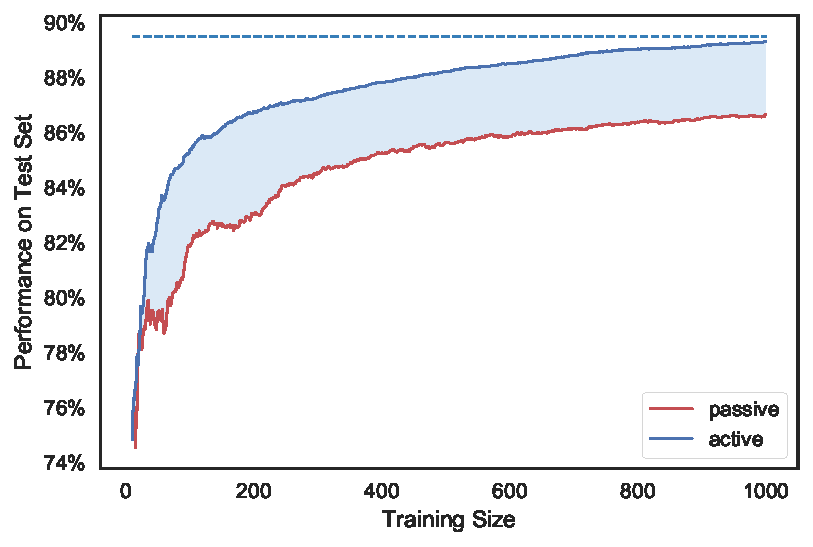
\includegraphics[width=0.7\textwidth]{figures/strength}
	\caption[Strength Measure]{An illustration of the strength measure. It is
	proportional to the shaded area between the (red) passive learning curve
	and the (blue) active learning curve. The bigger the area is, the more the
	active learner outperforms the passive learner. The top dotted line
	indicates the maximum performance achieved by using the entire labeled
	pool as training data.}
	\label{fig:strength}
\end{figure}

\section{Results and Discussion}\label{sec:discuss}

\subsection{Results}

Figure~\ref{fig:strengths-small} and~\ref{fig:strengths-large} show the
strengths of all methods that we consider, while
Figure~\ref{fig:learning_curves-small} and~\ref{fig:learning_curves-large}
provide selected learning curves. Plots for the 6 small datasets with fewer
than 500 examples (glass, ionosphere, iris, sonar, wine, and wpbc) are shown in
Figure~\ref{fig:strengths-small} and Figure~\ref{fig:learning_curves-small}.
Plots for the 2 medium-sized datasets (pima and vehicle) and the 4 large
datasets (magic, miniboone, pageblocks, and sdss) are shown in
Figure~\ref{fig:strengths-large} and Figure~\ref{fig:learning_curves-large}.
Each figure contains two subfigures, one reporting the raw accuracy score,
while the other showing the MPBA score.

We observe that with the small and medium-sized datasets, the effect of active
learning is minimal. The box plots for all of these datasets cross the zero
line, which means that there is no statistical difference between the
corresponding heuristic/combiner and passive learning. With the pima dataset,
active learning appears to perform better if we look at the raw accuracy score.
However from the MPBA score, where the class imbalance is taken into account,
the benefit starts to disappear. It is only with the 4 large datasets that
there is a visible gap between the passive learning curve and the active
learning curve for most methods. In fact, some of the gains are very
significant. In the sdss dataset, for example, the Borda method achieves an
MPBA of 87\% after only 200 labeled examples, while passive learning could only
reach the same performance after 1000 labeled examples (see
Figure~\ref{fig:learning_curves-mpba-large}).

Out of the 8 active learning heuristics tested, the heuristics with the
information density weighting (\textsc{w-confidence},
\textsc{w-margin}, and \textsc{w-entropy}) outperform passive learning only in
the pageblocks dataset (the most imbalanced dataset, with 90\% of the data
being in the majority class). \textsc{qbb-kl} performs slightly better in
pageblocks and miniboone. The remaining heuristics---\textsc{confidence},
\textsc{margin}, \textsc{entropy}, and \textsc{qbb-margin}---perform equally
well in magic, miniboone, pageblocks, and sdss.

We find no difference in performance between the bandit algorithms and
the rank aggregation methods. Combining active learners does not seem
to hurt the performance, even if we include a poorly performing heuristic
such as \textsc{qbb-kl}.

For bandit algorithms, it is interesting to note that \textsc{thompson}
favors certain heuristics a lot more than others, while the behavior of
\textsc{exp3++}, \textsc{ocucb}, and \textsc{klucb} is almost indistinguishable
from \textsc{explore}, where we explore 100\% of the time (see
Figure~\ref{fig:selection}).

\subsection{Discussion}

The experimental results allow us to answer the following questions:

\begin{enumerate}
	\item \textbf{Can active learning beat passive learning?} Yes, active
	learning can perform much better than passive learning when the unlabeled
	pool is large (e.g. sdss, miniboone, pageblock). When the dataset is small,
	we do not actually need active learning, since we can manually label
	everything.

	\item \textbf{Can active learning degrade performance?} Yes, there is no
	guarantee that active learning will always beat passive learning. For
	example, \textsc{w-entropy} actually slows down the learning in the magic
	dataset. However, this only happens with certain heuristics, like when the
	information density weighting is used.

	\item \textbf{What is the best single active learning heuristic?} All of
	\textsc{confidence}, \textsc{margin}, \textsc{entropy}, and
	\textsc{qbb-margin} have a similar performance. However \textsc{confidence}
	is perhaps the simplest to compute and thus is a good default choice in
	practice.

	\item \textbf{What are the challenges in using bandit algorithms?}
	\begin{enumerate}
		\item Designing a good reward scheme is difficult. This paper uses the
		increase in the classifier performance as the reward. However this type
		of reward is non-stationary (i.e. it gets smaller after each step as
		learning saturates) and the rewards will thus eventually go to zero.
		\item In practice, we do not have a representative test set that can be
		used to compute the reward. As a workaround, \cite{hsu15} computed the
		reward on the training set and then used importance weighting to remove
		any potential bias. For this to work, we need to ensure that every
		training example and every active learning suggestion have a non-zero
		probability of being selected in each step.
		\item Finally, some bandit algorithms such as Thompson sampling
		require that the reward follows a certain distribution (e.g. Gaussian).
		This can be hard to satisfy.
	\end{enumerate}

	\item \textbf{What are the challenges in using rank aggregation
	algorithms?}
	\begin{enumerate}
		\item We need to compute the scores from all heuristics at every time
		step. This might not be feasible if there are too many heuristics or if
		we include heuristics that require a large amount of compute power
		(e.g. variance minimization).
		\item The Schulze method uses $O(n^2)$ space, where $n$ is the number
		of candidates. This might lead to memory issues if we need to rank
		a large number of candidates from the unlabeled pool.
		\item Before aggregating the rankings, we throw away the score
		magnitudes, which could cause a loss of information.
		\item Unlike bandit algorithms, all of the rank aggregators always give
		each heuristic an equal weight.
	\end{enumerate}

	\item \textbf{Which method should I use in practice to combine active
	learners?} Since there is no difference in performance between various
	combiners,  we recommend using a simple rank aggregator like Borda count or
	geometric mean if we do not want to select a heuristic a priori. Rank
	aggregators do not need a notion of a reward---we simply give all
	suggestions an equal weight when combining. Thus we neither need to a keep
	a separate test set, nor do we need to worry about designing a good reward
	scheme.
\end{enumerate}

\section{Conclusion}

In this paper we empirically compared 16 active learning methods with passive
learning. Using benchmark datasets, we found that active learning can reduce
the training set size considerably, especially when we have a lot of unlabeled
data. Combining active learners with bandit and rank aggregation methods does
not in general degrade the performance. In particular, Borda count and the
geometric mean are good practical algorithms given their simplicity and the
fact that we do not have to design a reward scheme.

\begin{figure}[tbp]
	\centering
	\begin{subfigure}[t]{\textwidth}
        \centering
        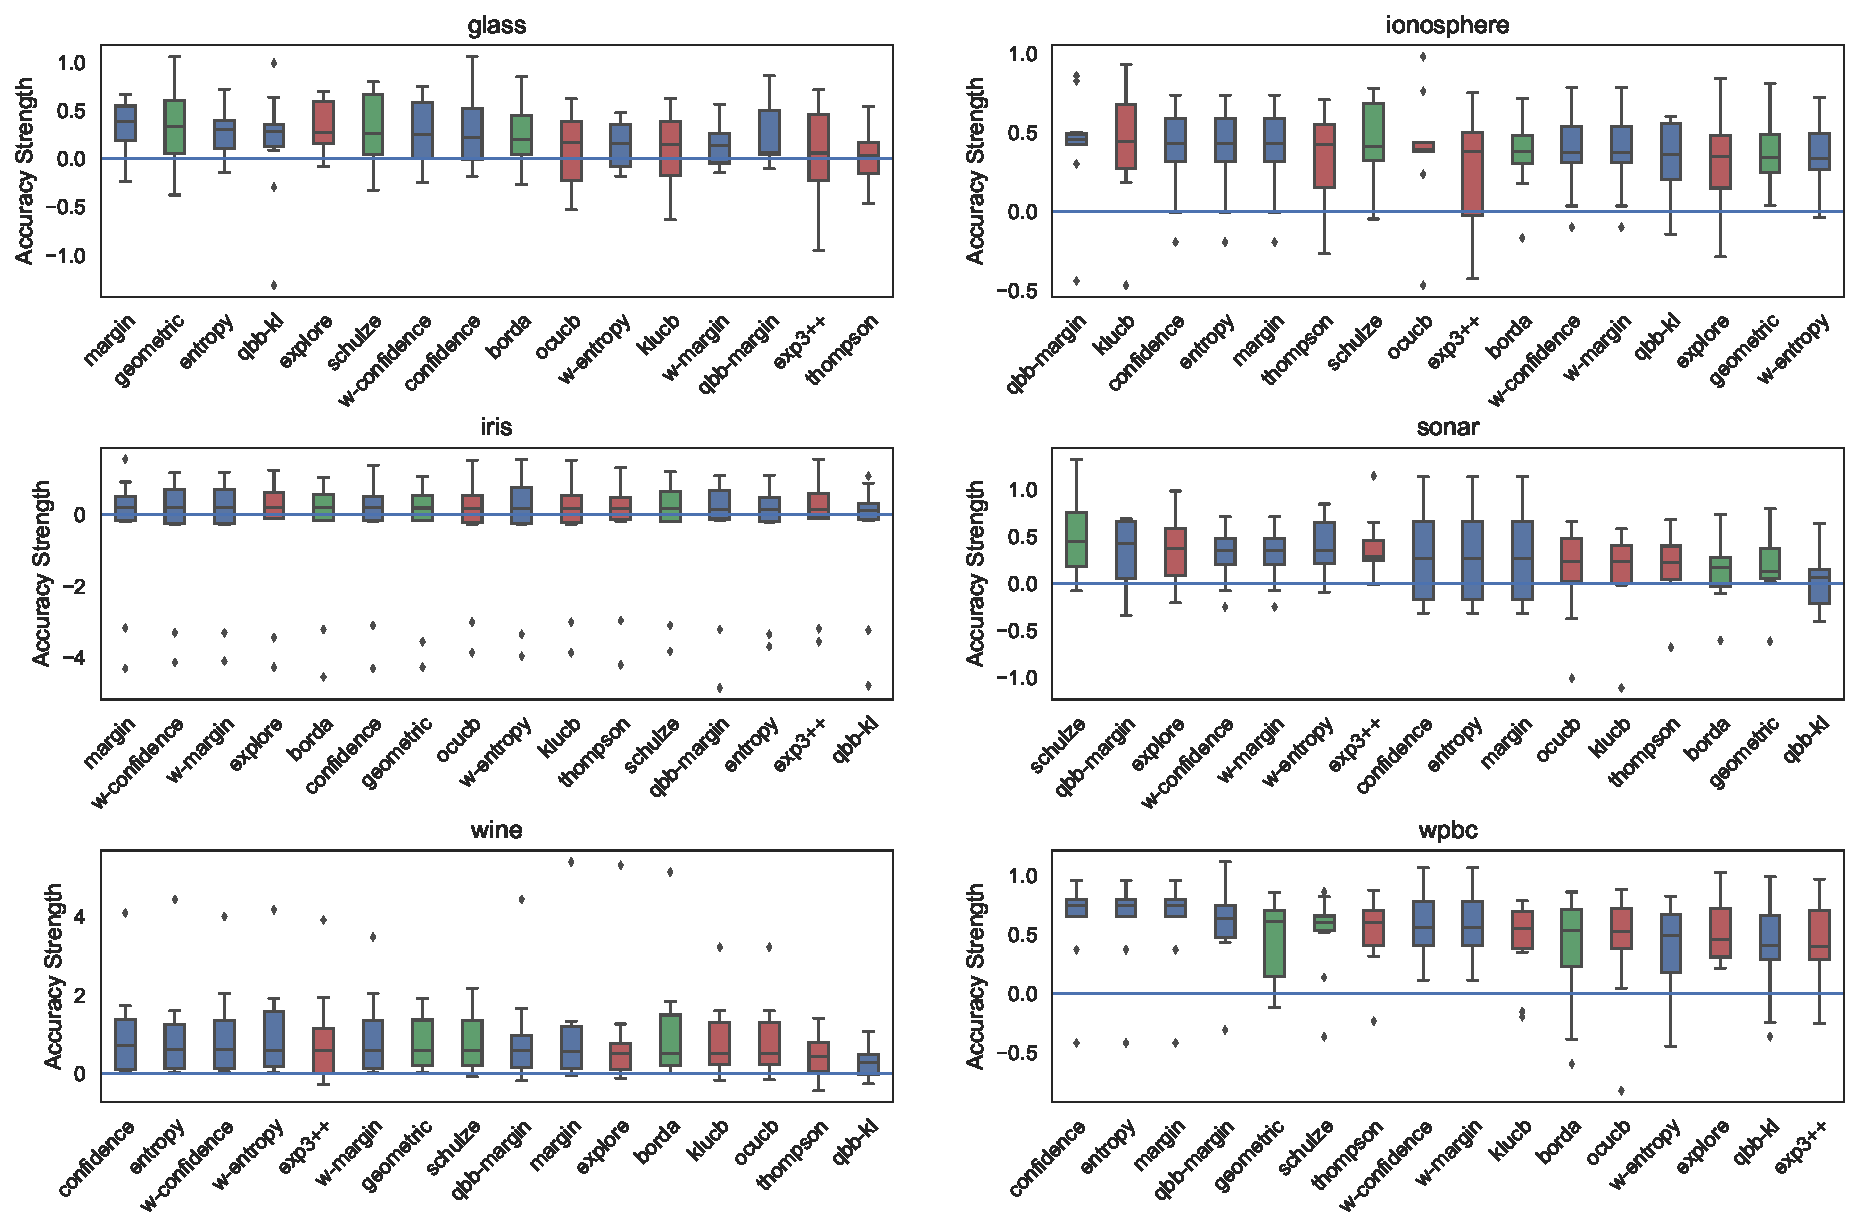
\includegraphics[width=\textwidth]{figures/strengths-accuracy-small}
		\caption{Accuracy strength}
		\label{fig:strengths-accuracy-small}
	\end{subfigure}
	\begin{subfigure}[t]{\textwidth}
        \centering
        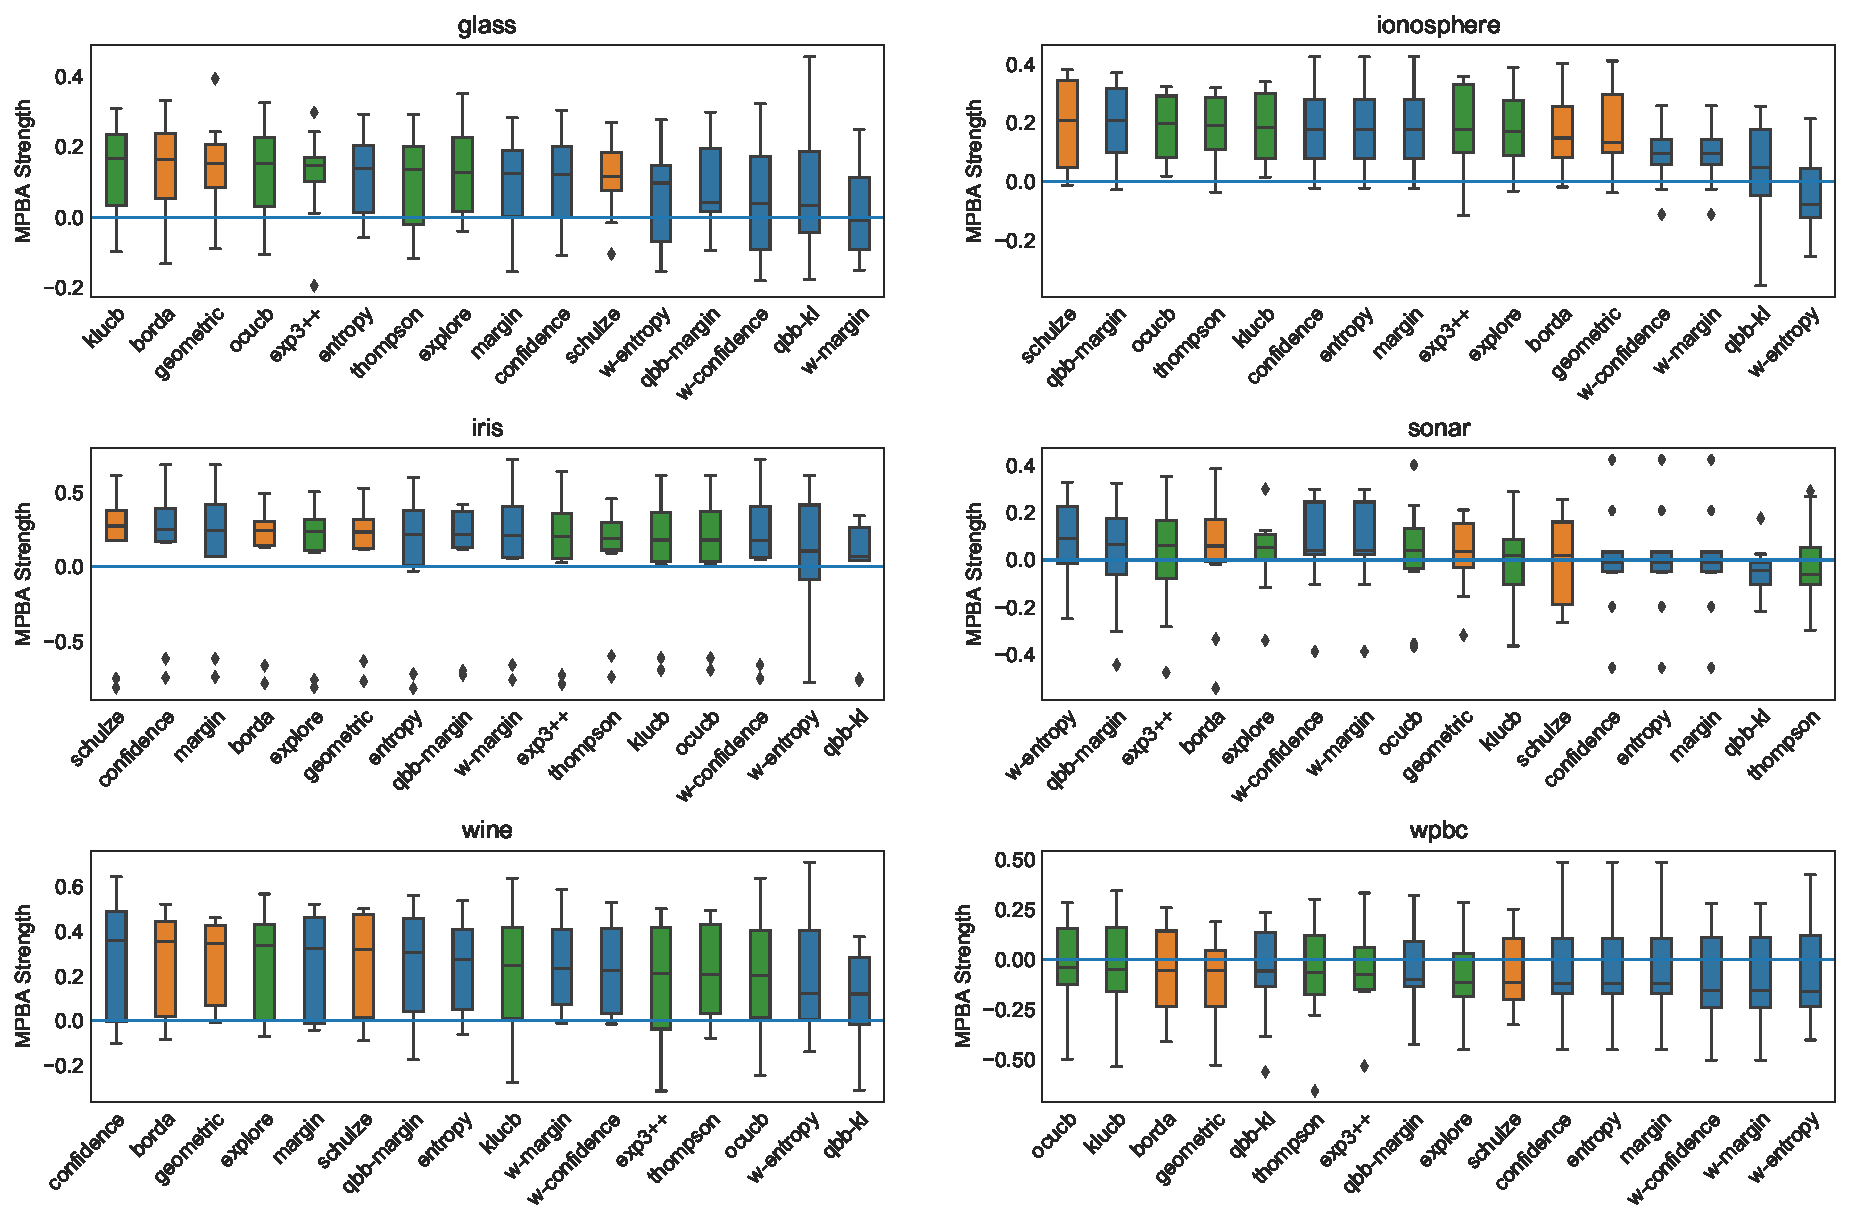
\includegraphics[width=\textwidth]{figures/strengths-mpba-small}
		\caption{MPBA strength}
		\label{fig:strengths-accuracy-large}
    \end{subfigure}
	\caption[Policy strength]{Boxplots of the accuracy and MPBA strength of the
	16 active learning strategies, relative to passive learning, using the
	small datasets (glass, ionosphere, iris, sonar, wine, and wpbc). The more
	positive the strength is, the better the heuristic/combiner is. Blue boxes
	represent individual heuristics; red boxes represent bandit algorithms, and
	green boxes are for rank aggregation methods. A strategy that is above the
	zero line is better than passive learning. Each boxplot contains 10 trials.
	The accuracy score is a simple metric that simply counts up the number of
	correct predictions. The MPBA score, being the average of the recall, gives
	an equal representation to each class.}
	\label{fig:strengths-small}
\end{figure}

\begin{figure}[tbp]
	\centering
	\begin{subfigure}[t]{\textwidth}
        \centering
        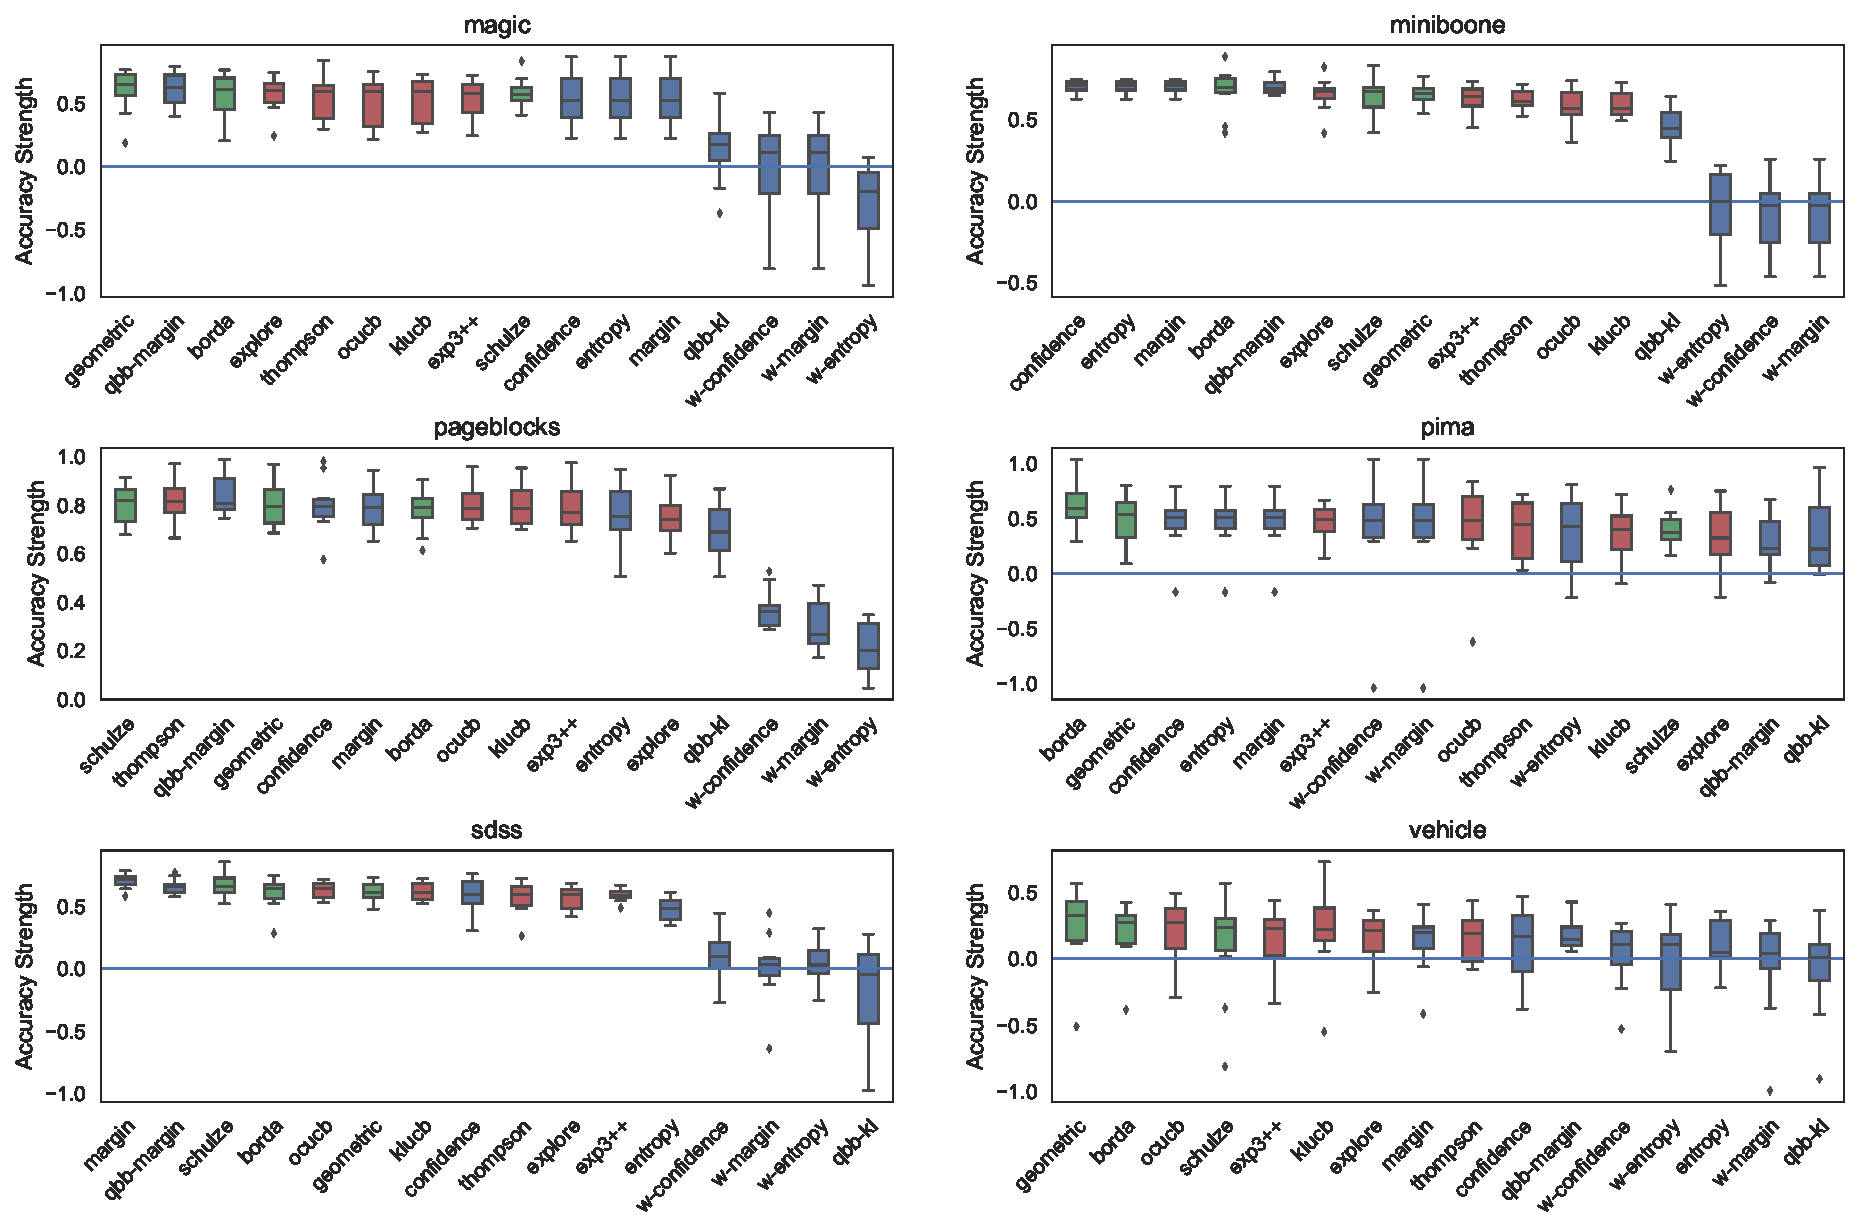
\includegraphics[width=\textwidth]{figures/strengths-accuracy-large}
		\caption{Accuracy strength}
		\label{fig:strengths-mpba-small}
	\end{subfigure}
	\begin{subfigure}[t]{\textwidth}
        \centering
        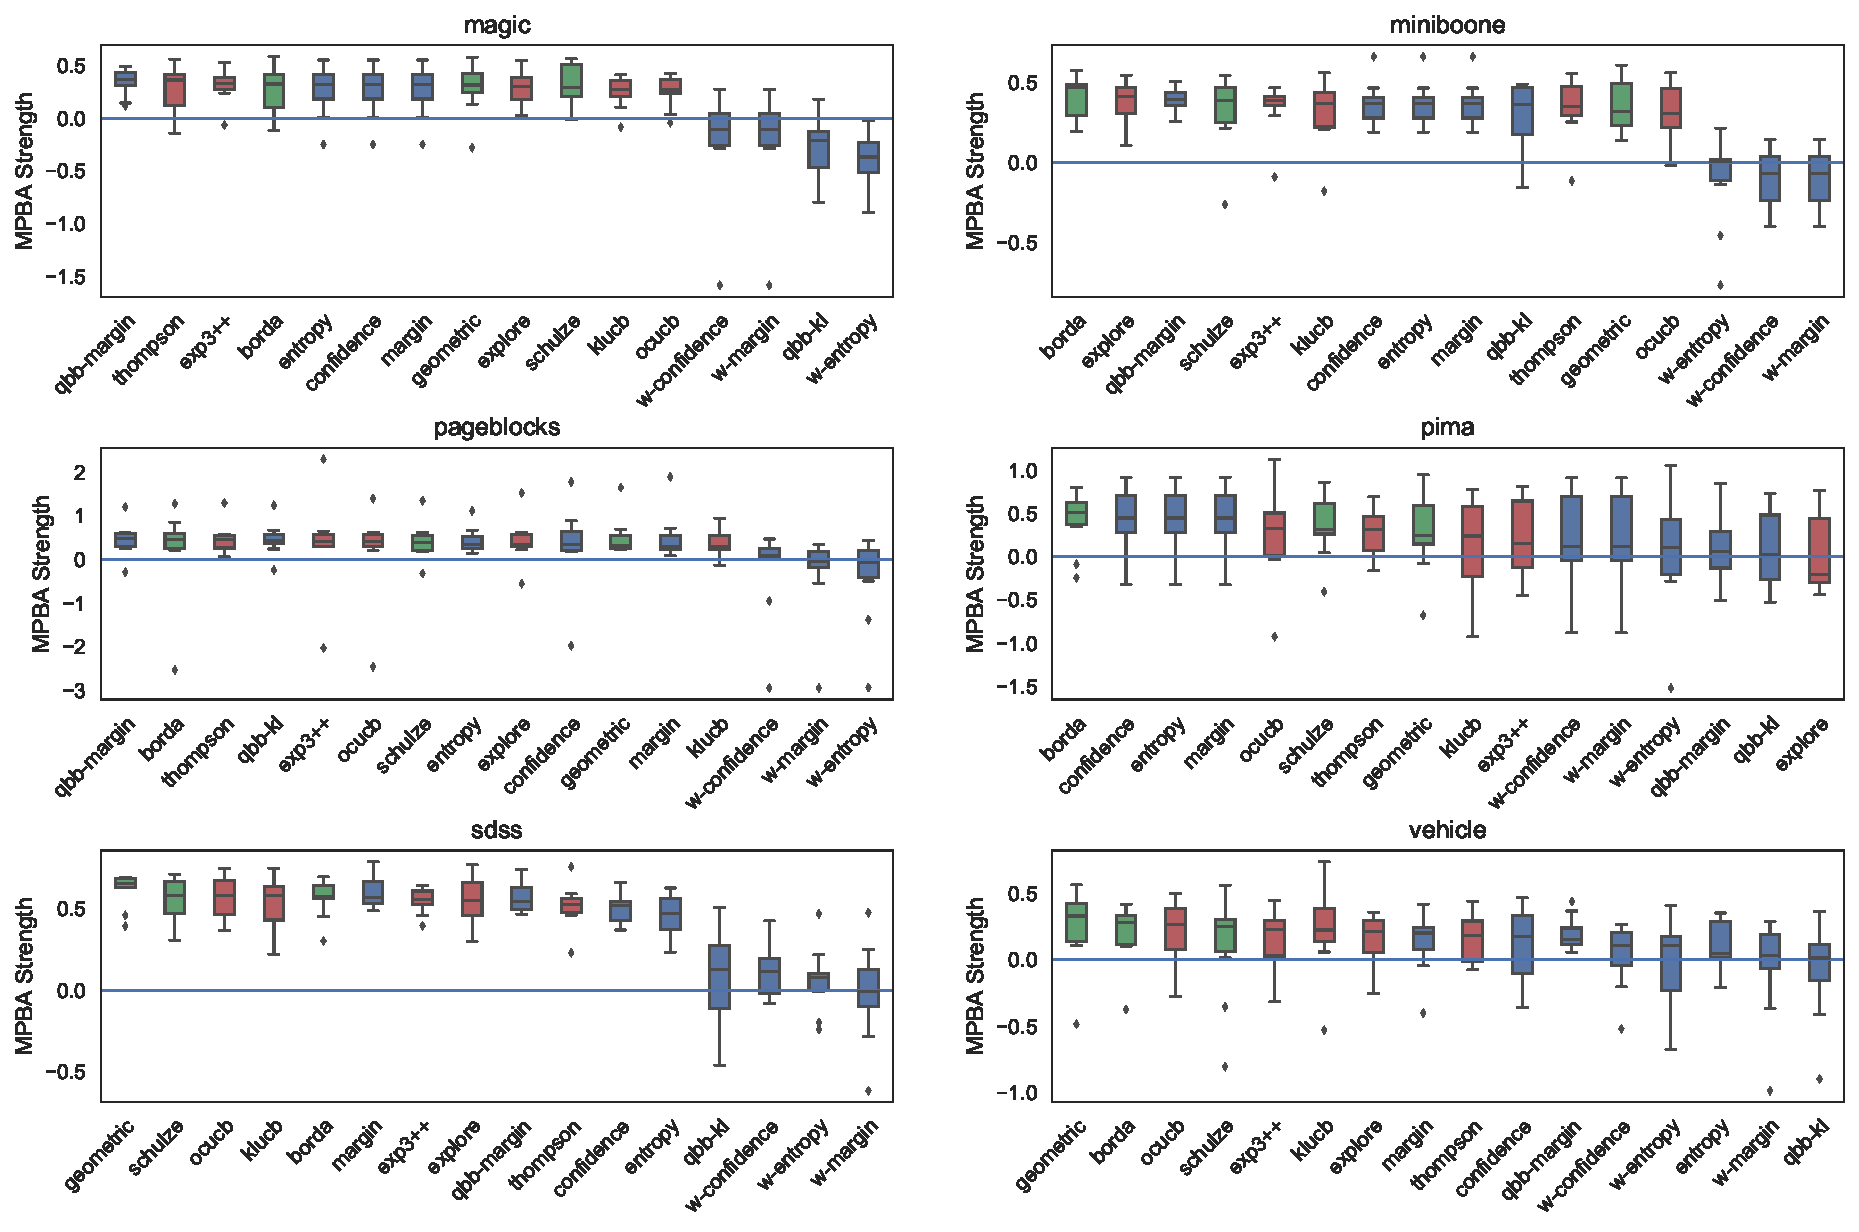
\includegraphics[width=\textwidth]{figures/strengths-mpba-large}
		\caption{MPBA strength}
		\label{fig:strengths-mpba-large}
    \end{subfigure}
	\caption[Policy strength]{Boxplots of the accuracy and MPBA strength of the
	16 active learning strategies, relative to passive learning, using the
	medium-to-large datasets (magic, miniboone, pageblocks, pima, sdss, and
	vehicle). The more positive the strength is, the better the
	heuristic/combiner is. Blue boxes represent individual heuristics; red
	boxes represent bandit algorithms, and green boxes are for rank aggregation
	methods. A strategy that is above the zero line is better than passive
	learning. Each boxplot contains 10 trials. The accuracy score is a simple
	metric that simply counts up the number of correct predictions. The MPBA
	score, being the weighted average of the recall, gives an equal
	representation to each class.}
	\label{fig:strengths-large}
\end{figure}


\begin{figure}[tbp]
	\centering
	\begin{subfigure}[t]{\textwidth}
        \centering
        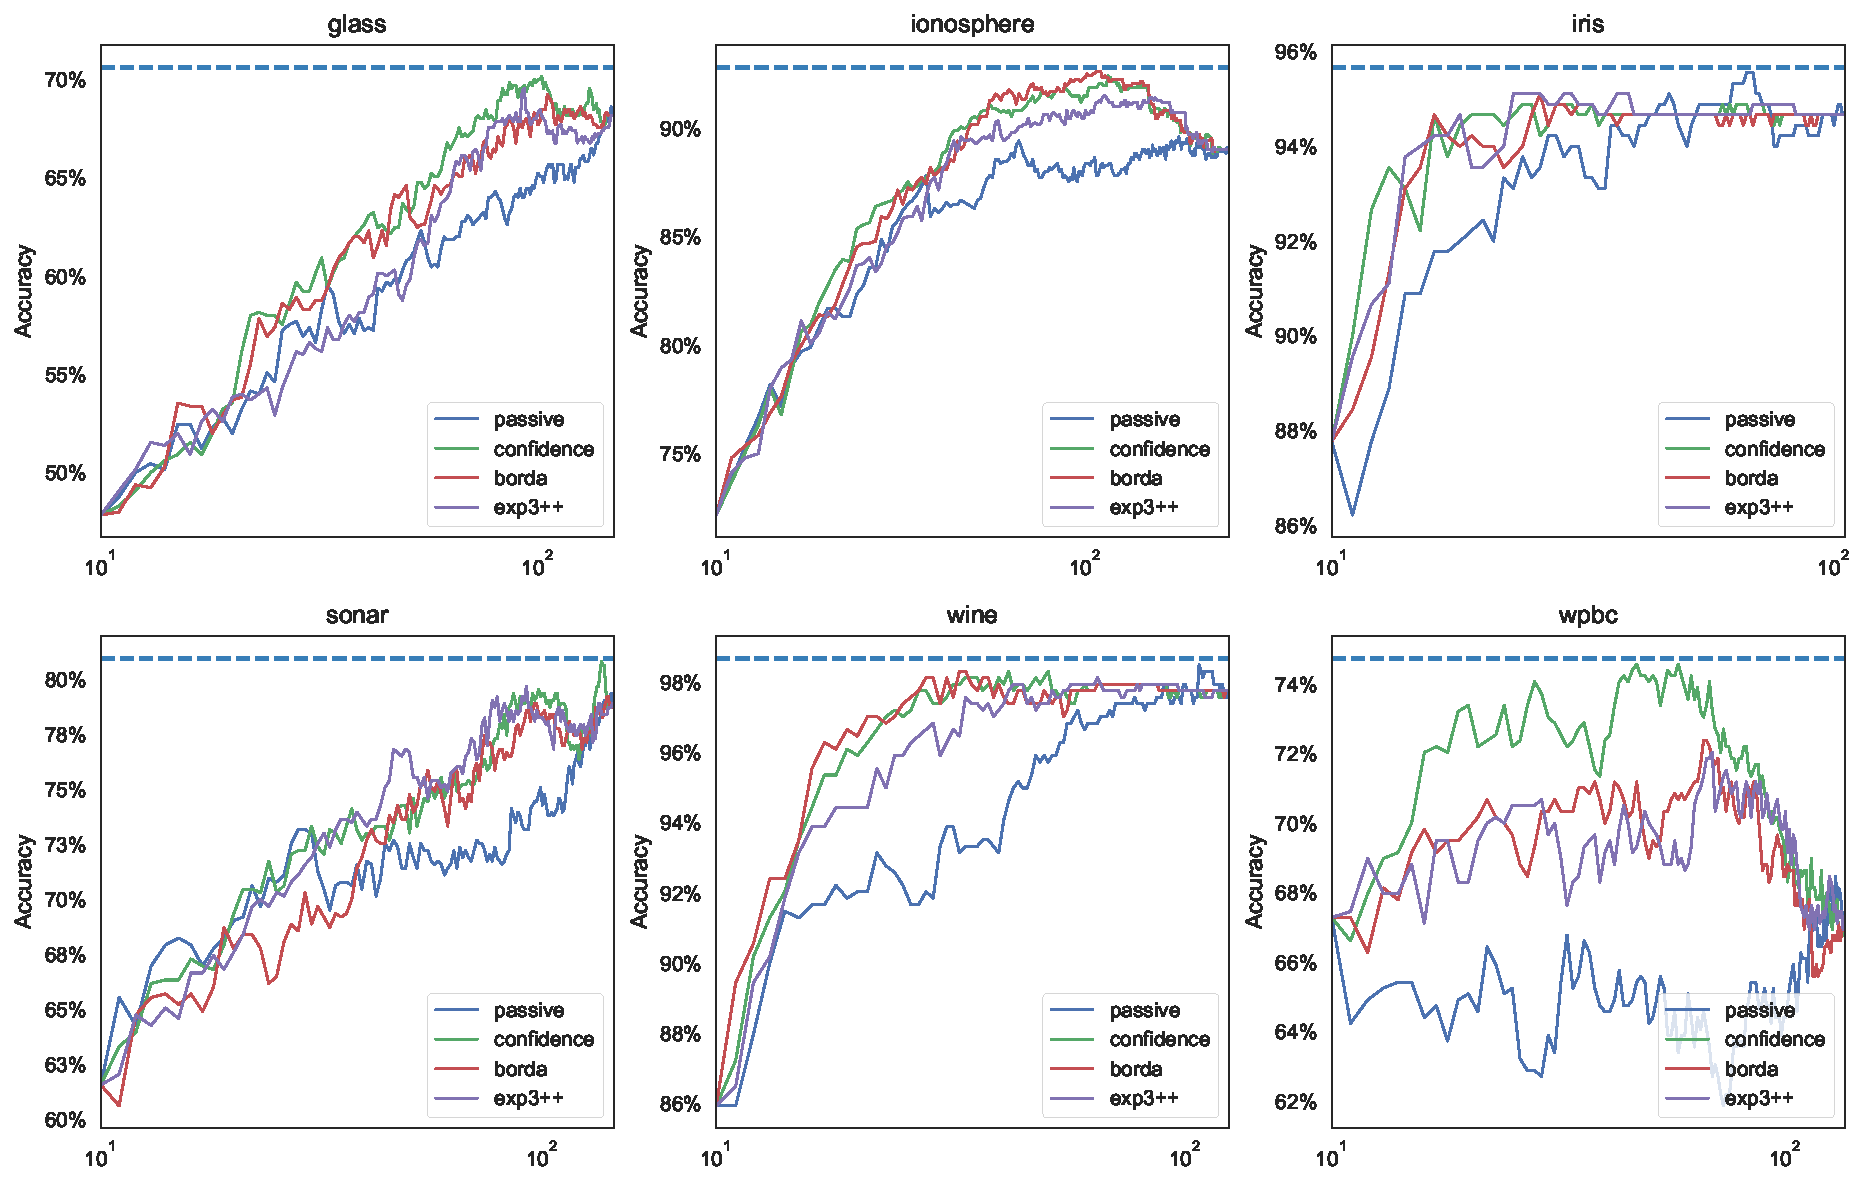
\includegraphics[width=\textwidth]{figures/learning_curves-accuracy-small}
		\caption{Accuracy learning curves}
		\label{fig:learning_curves-accuracy-small}
	\end{subfigure}
	\begin{subfigure}[t]{\textwidth}
        \centering
        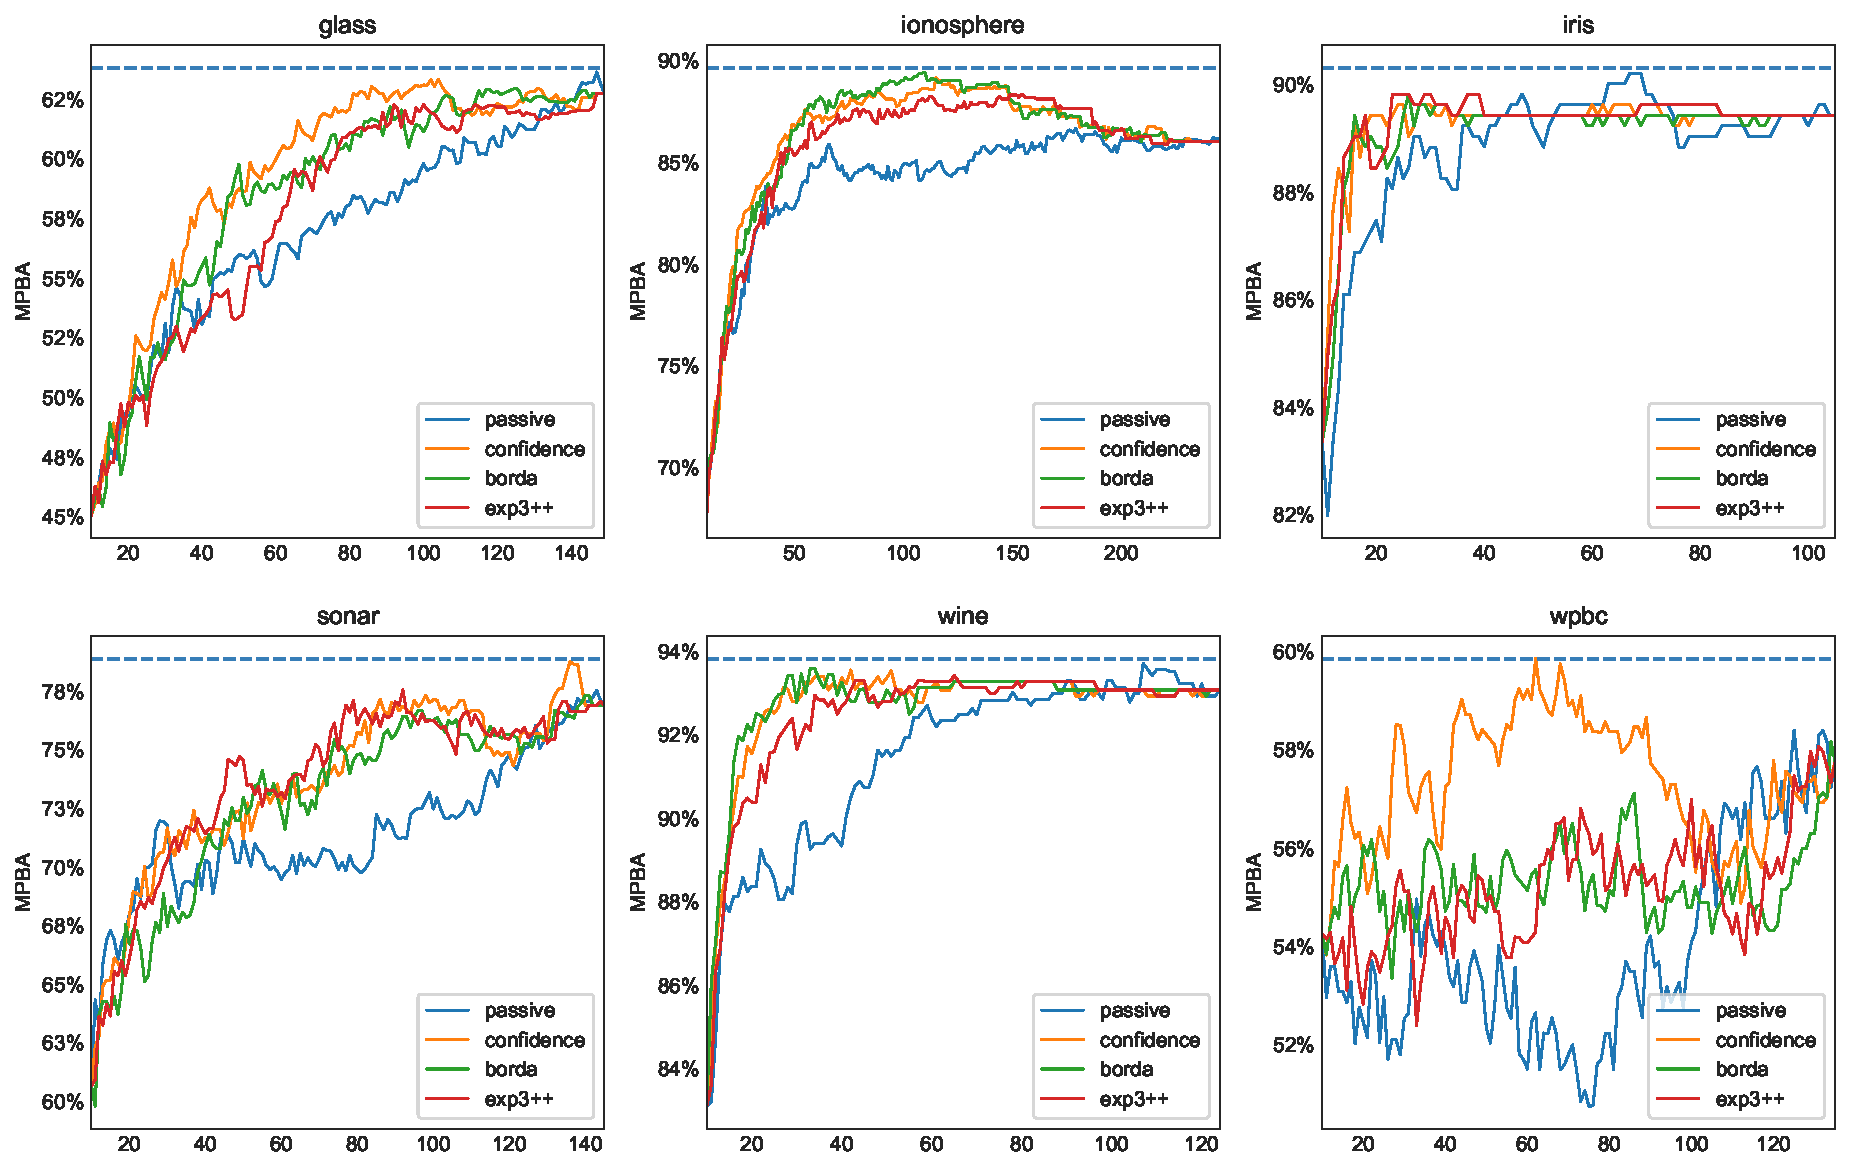
\includegraphics[width=\textwidth]{figures/learning_curves-mpba-small}
		\caption{MPBA learning curves}
		\label{fig:learning_curves-accuracy-large}
    \end{subfigure}
	\caption[Selected learning curves]{Selected accuracy and MPBA learning
	curves for the small datasets (glass, ionosphere, iris, sonar, wine, and
	wpbc). As it would get too cluttered to plot 17 learning curves, we only
	show the learning curve for \textsc{passive}, \textsc{confidence},
	\textsc{exp3++}, and \textsc{borda}. The learning curves are averaged over
	10 trials.}
	\label{fig:learning_curves-small}
\end{figure}

\begin{figure}[tbp]
	\centering
	\begin{subfigure}[t]{\textwidth}
        \centering
        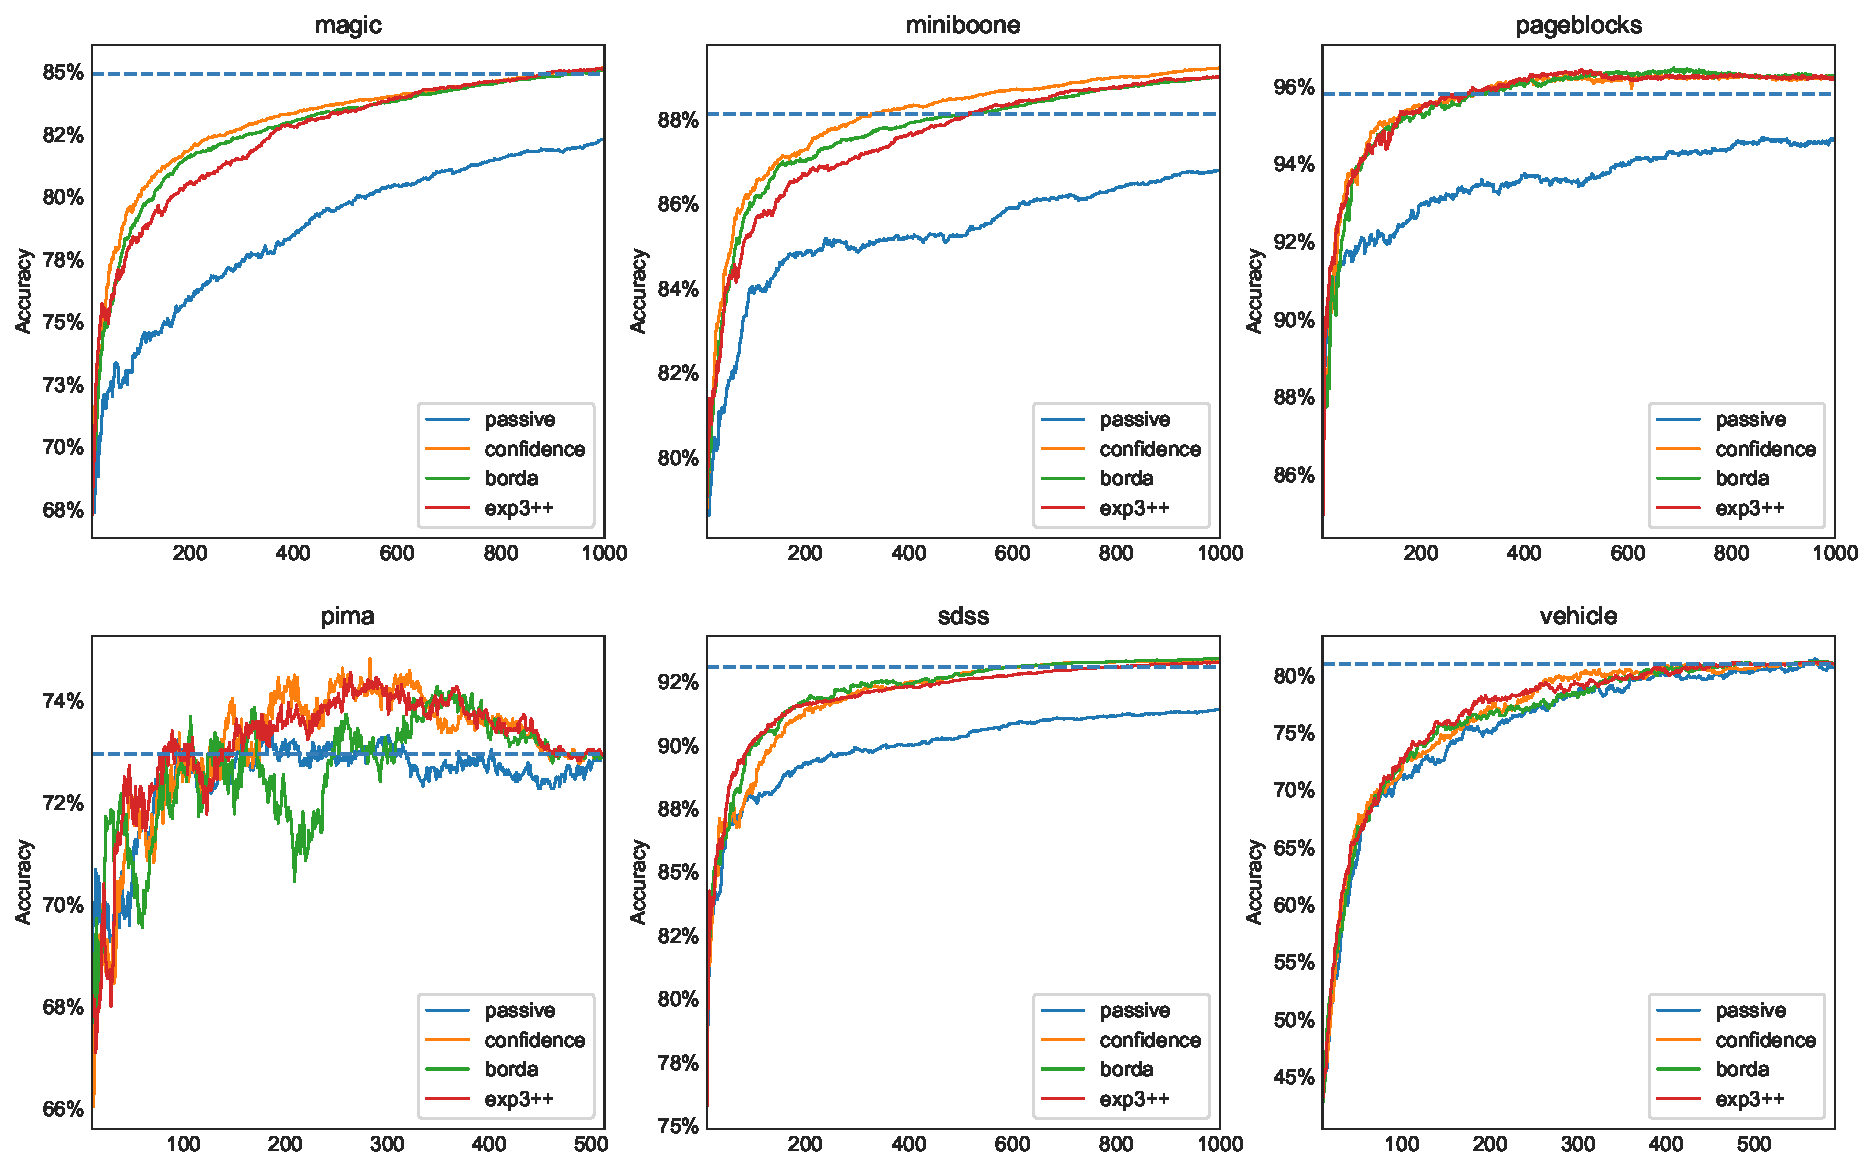
\includegraphics[width=\textwidth]{figures/learning_curves-accuracy-large}
		\caption{Accuracy learning curves}
		\label{fig:learning_curves-mpba-small}
	\end{subfigure}
	\begin{subfigure}[t]{\textwidth}
        \centering
        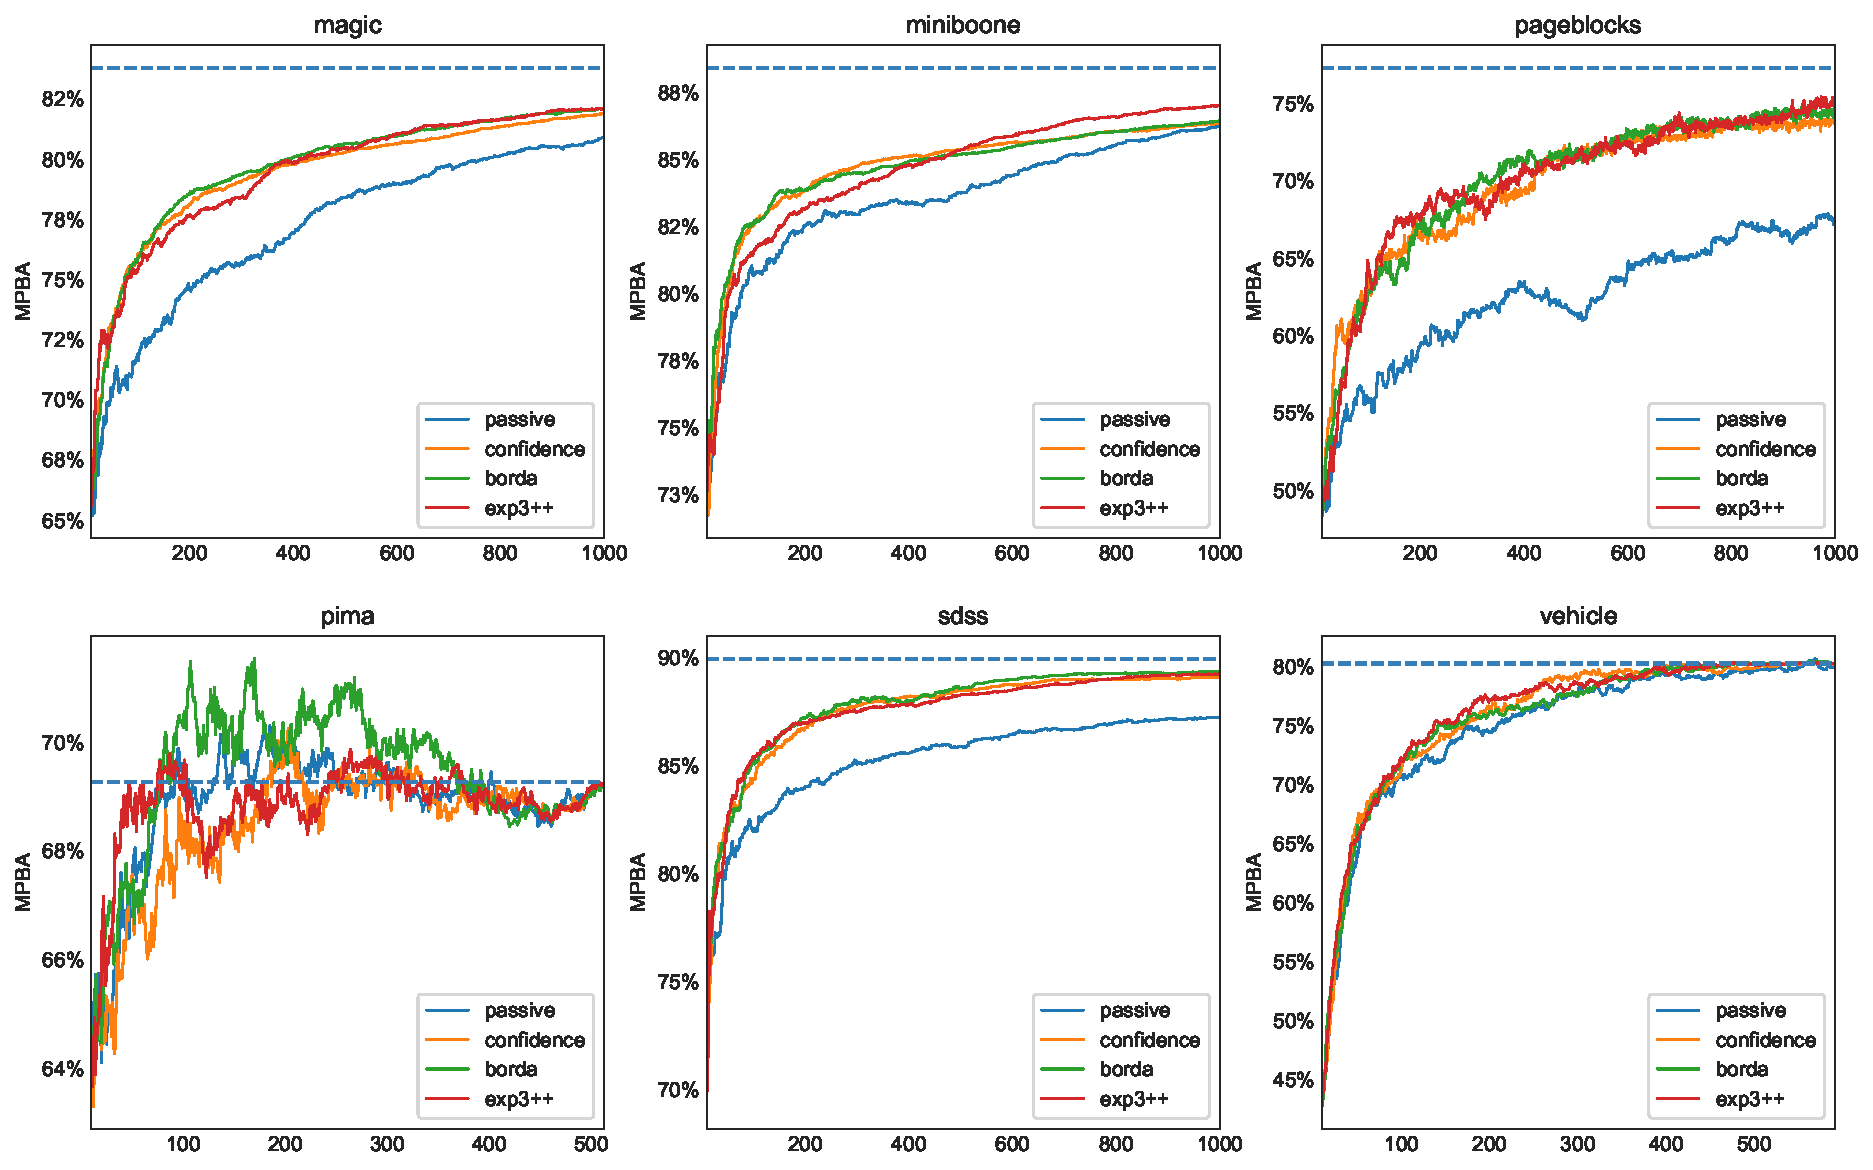
\includegraphics[width=\textwidth]{figures/learning_curves-mpba-large}
		\caption{MPBA learning curves}
		\label{fig:learning_curves-mpba-large}
    \end{subfigure}
	\caption[Selected learning curves]{Selected accuracy and MPBA learning
	curves for the medium-to-large datasets (magic, miniboone, pageblocks,
	pima, sdss, and vehicle). As it would get too cluttered to plot 17 learning
	curves, we only show the learning curve for \textsc{passive},
	\textsc{confidence}, \textsc{exp3++}, and \textsc{borda}. The learning
	curves are averaged over 10 trials.}
	\label{fig:learning_curves-large}
\end{figure}

\begin{figure}[tbp]
	\centering
	\begin{subfigure}[t]{\textwidth}
        \centering
        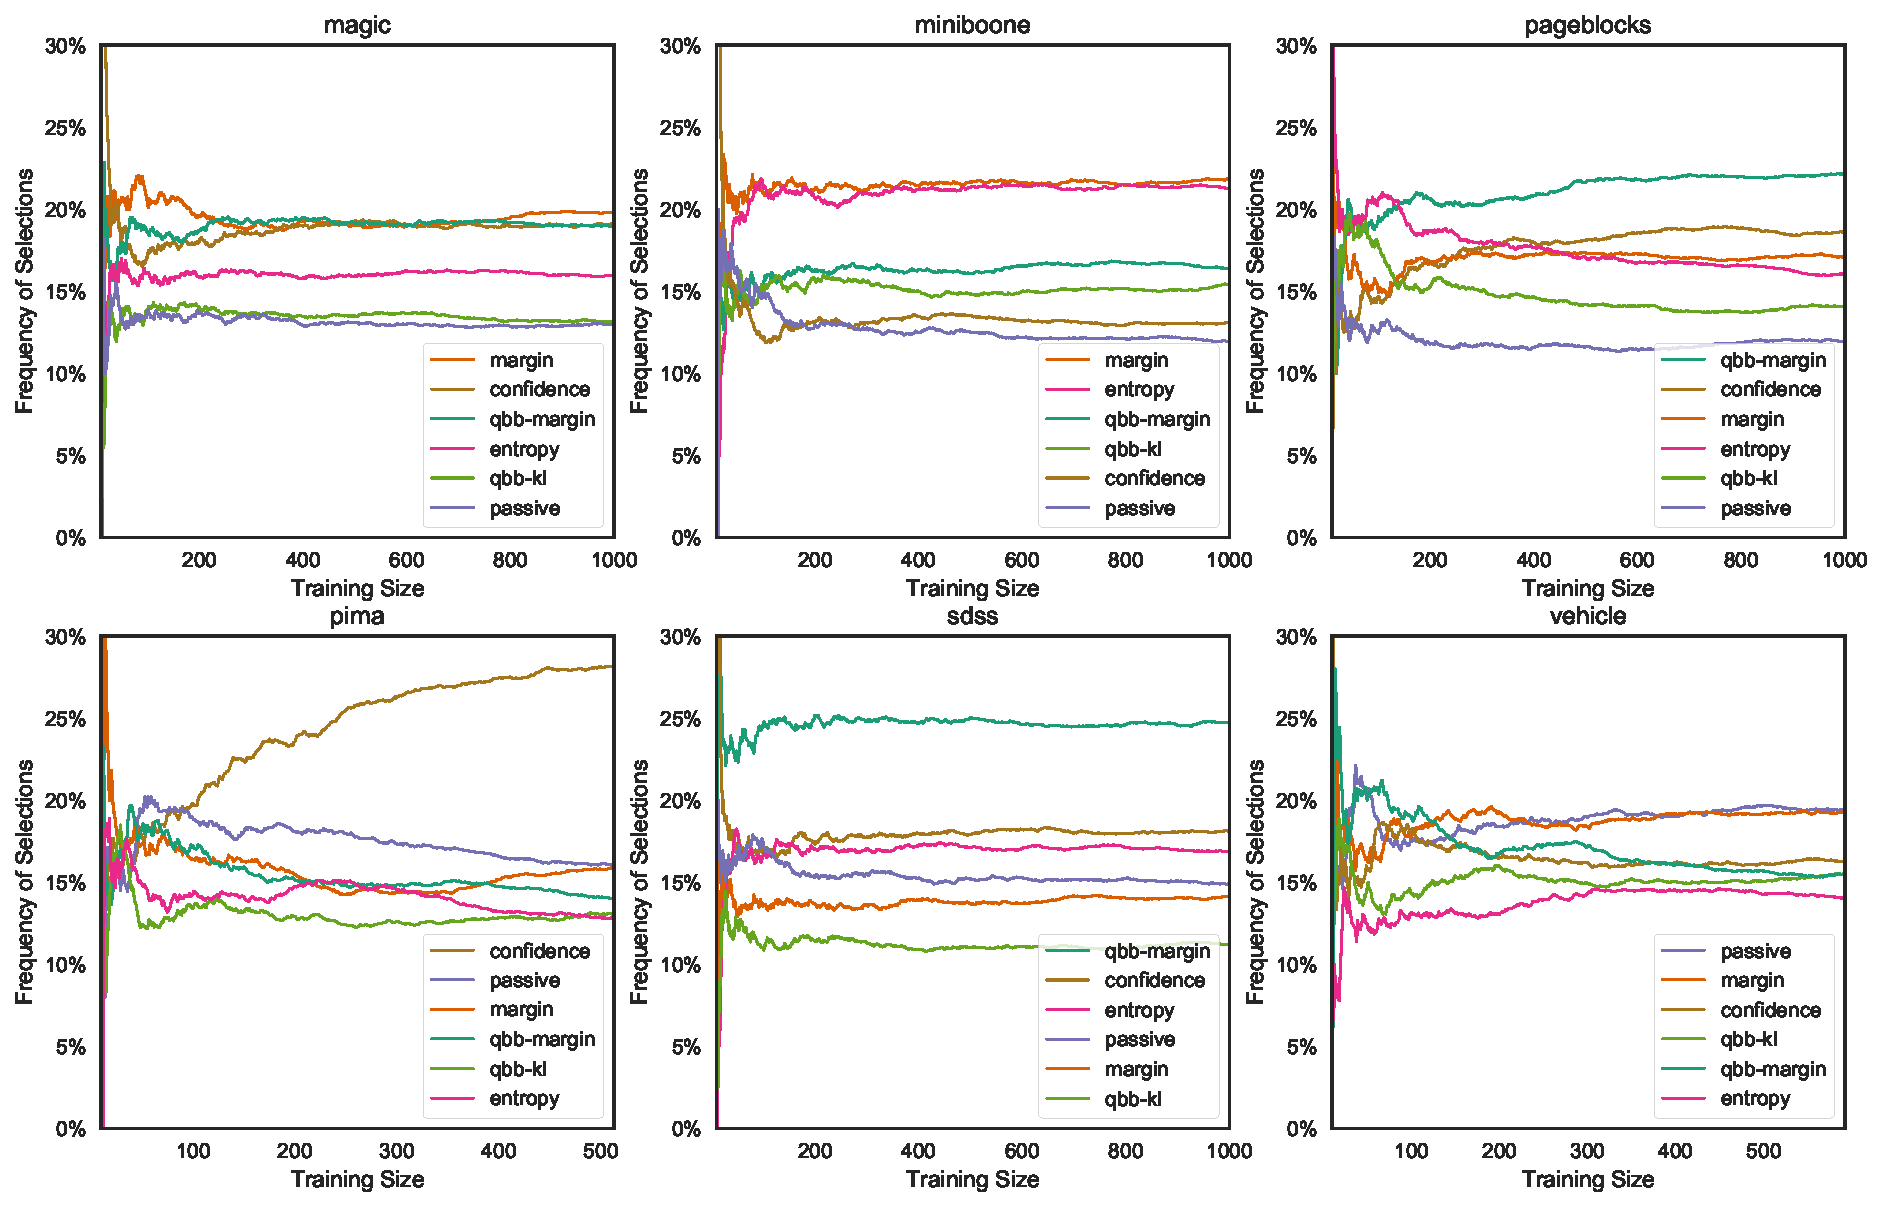
\includegraphics[width=\textwidth]{figures/selection-thompson-large}
		\caption{Thompson sampling}
		\label{fig:selection-thompson-large}
	\end{subfigure}
	\begin{subfigure}[t]{\textwidth}
        \centering
        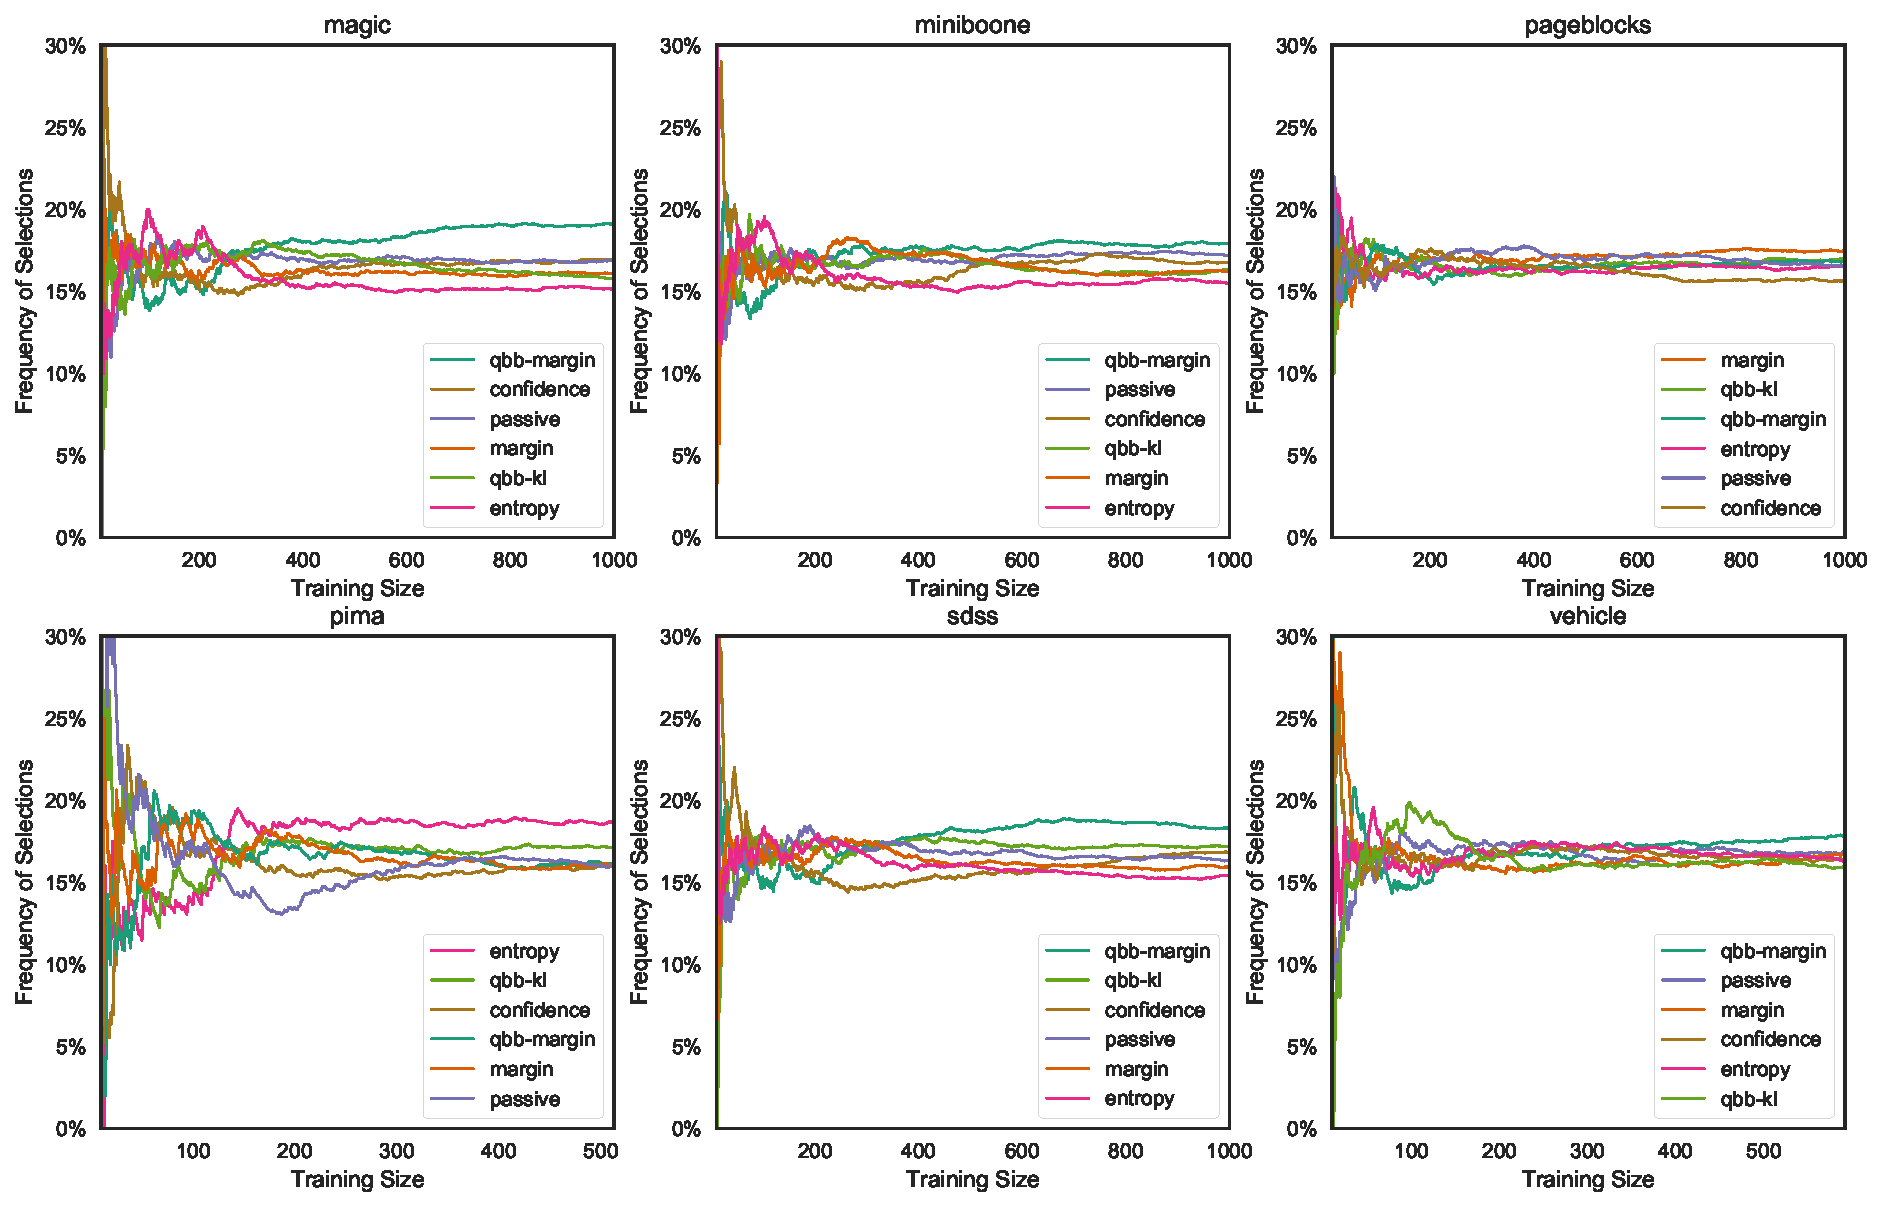
\includegraphics[width=\textwidth]{figures/selection-exp++-large}
		\caption{EXP3++ algorithm}
		\label{fig:selection-exp-large}
    \end{subfigure}
	\caption[Heuristic selection frequencies]{Selection frequencies of
	heuristics in \textsc{thompson} and \textsc{exp3++}, with the large
	datasets (magic, miniboone, pageblocks, pima, sdss, and vehicle). The plots
	show how often each of the heuristics gets selected over time. The
	selection frequencies are averaged over 10 trials. \textsc{thompson} favors
	certain heuristics more strongly than others. In contrast, \textsc{exp3++}
	favors uniform exploration more, sampling each heuristic with roughly equal
	weights. The plots for \textsc{ocucb} and \textsc{klucb} are not shown
	here, but they are similar to \textsc{exp3++}.}
	\label{fig:selection}
\end{figure}


\section{Acknowledgments}

The research was supported by the Data to Decisions Cooperative Research
Centre whose activities are funded by the Australian Commonwealth Government’s
Cooperative Research Centres Programme.

This research was supported by the Australian Research Council Centre of
Excellence for All-sky Astrophysics (CAASTRO), through project number
CE110001020.

The UCI datasets were downloaded from the UCI Machine Learning
Repository\footnote{\url{http://archive.ics.uci.edu/ml}}. In particular, the
vehicle
dataset\footnote{\url{https://archive.ics.uci.edu/ml/datasets/Statlog+(Vehicle+Silhouettes)}}
comes from the Turing Institute, Glasgow, Scotland.

The SDSS dataset\footnote{\url{http://dx.doi.org/10.5281/zenodo.58500}} was
extracted from Data Release 12 of SDSS-III. Funding for SDSS-III has been
provided by the Alfred P. Sloan Foundation, the Participating Institutions, the
National Science Foundation, and the U.S. Department of Energy Office of
Science. The SDSS-III web site is http://www.sdss3.org/.

SDSS-III is managed by the Astrophysical Research Consortium for the
Participating Institutions of the SDSS-III Collaboration including the
University of Arizona, the Brazilian Participation Group, Brookhaven National
Laboratory, Carnegie Mellon University, University of Florida, the French
Participation Group, the German Participation Group, Harvard University, the
Instituto de Astrofisica de Canarias, the Michigan State/Notre Dame/JINA
Participation Group, Johns Hopkins University, Lawrence Berkeley National
Laboratory, Max Planck Institute for Astrophysics, Max Planck Institute for
Extraterrestrial Physics, New Mexico State University, New York University,
Ohio State University, Pennsylvania State University, University of Portsmouth,
Princeton University, the Spanish Participation Group, University of Tokyo,
University of Utah, Vanderbilt University, University of Virginia, University
of Washington, and Yale University.



\bibliography{active}

\pagebreak

\section*{Appendix A: Posterior Balanced Accuracy}


Most real-world datasets are unbalanced. In the SDSS dataset, for example,
there are 4.5 times as many galaxies as quasars. The problem of class imbalance
is even more severe in the pageblocks dataset, where one class makes up 90\% of
the data and the remaining four classes only make up 10\%. An easy fix is to
undersample the dominant class when creating the training and test sets. This,
of course, means that the size of these sets is limited by the size of the
minority class.

When we do not want to alter the underlying class distribution or when larger
training and test sets are desired, we need a performance measure that can
correct for the class imbalance.~\cite{brodersen10} showed that the posterior
balanced accuracy distribution can overcome the bias in the binary case. We now
extend this idea to the multi-class setting.

Suppose we have $k$ classes. For each class $i$ between $1$ and $k$, there are
$N_i$ objects in the universe. Given a classifier, we can predict the label of
every object and compare our prediction with the true label. Let $G_i$ be the
number of objects in class $i$ that are correctly predicted.
Then we define the recall $A_i$ of class $i$ as\index{recall}
	\begin{IEEEeqnarray}{lCl}
		A_i &=& \frac{G_i}{N_i}
	\end{IEEEeqnarray}
The problem is that it is not feasible to get the actual values of $G_i$ and
$N_i$ since that would require us to obtain the true label of every object in
the universe. Thus we need a method to estimate these quantities when we only
have a sample. Initially we have no information about $G_i$ and $N_i$, so we
can assume that each $A_i$ follows a uniform prior distribution between 0 and
1. This is the same as a Beta distribution with shape parameters $\alpha =
\beta = 1$:
	\begin{IEEEeqnarray}{lCl}
		A_i &\sim& \Beta(1,1)
	\end{IEEEeqnarray}
The probability density function (PDF) of $A_i$ is then
    \begin{IEEEeqnarray}{lCl}
        f_{A_i}(a) &=& \frac{\Gamma(\alpha+\beta)}{\Gamma(\alpha)\Gamma(\beta)}\,
        a^{\alpha-1}(1-a)^{\beta-1} \label{eqn:prior} \\
        &\propto&   a^{1-1}(1-a)^{1-1}  \notag
    \end{IEEEeqnarray}
where $\Gamma(\alpha)$ is the gamma function.

After we have trained the classifier, suppose we have a test set containing
$n_i$ objects in class $i$. Running the classifier on this test set is the same
as conducting $k$ binomial experiments, where, in the $i$th experiment, the
sample size is $n_i$ and the probability of success is simply $A_i$. Let $g_i$
be the number of correctly labeled objects belonging to class $i$ in the test
set. Then, conditional on the recall rate $A_i$, $g_i$ follows a binomial
distribution:
	\begin{IEEEeqnarray}{lCl}
		(g_i \mid A_i) &\sim& \Bin(n_i, A_i)
	\end{IEEEeqnarray}
The probability mass function of $(g_i \mid A_i = a)$ is thus
    \begin{IEEEeqnarray}{lCl}
		p_{g_i \mid A_i}(g_i) &=& \binom{n_i}{g_i} a^{g_i} (1 - a)^{n_i - g_i}
						  							\label{eqn:likelihood} \\
                              &\propto& a^{g_i} (1 - a)^{n_i - g_i} \notag
    \end{IEEEeqnarray}
In the Bayesian \index{Bayesian} setting, Eq. ~\eqref{eqn:prior} is the prior
and Eq. \eqref{eqn:likelihood} is the likelihood. To get the posterior PDF, we
simply multiply the prior with the likelihood:
	\begin{IEEEeqnarray}{lCl}
		f_{A_i \mid \bm{g}}(a)
		&\propto& f_{A_i}(a) \times f_{g_i \mid A_i}(g_i) \\
		&\propto& a^{1-1}(1-a)^{1-1} \times a^{g_i} (1 - a)^{n_i - g_i} \\
		&=& a^{1 + g_i - 1}(1-a)^{1 + n_i - g_i - 1}
	\end{IEEEeqnarray}
Thus, with respect to the binomial likelihood function,
the Beta distribution is conjugate to itself. The posterior recall rate $A_i$
also follows a Beta distribution, now with parameters
	\begin{IEEEeqnarray}{lCl}
		(A_i \mid g_i) &\sim& \Beta(1 + g_i, 1 + n_i - g_i)
	\end{IEEEeqnarray}
Our goal is to have a balanced accuracy rate, $A$, that puts an equal weight in
each class. One way to achieve this is to take the average of the individual
recalls:
	\begin{IEEEeqnarray}{lCl}
		A &=& \frac{1}{k} \sum_{i=1}^k A_i \\
		&=& \frac{1}{k} A_T
	\end{IEEEeqnarray}
Here we have defined $A_T$ to be the sum of the individual recalls. We call $(A
\mid \bm{g})$ the posterior balanced accuracy, where $\bm{g} =(g_1,...,g_k)$.
Most of the time, we simply want to calculate its expected value:
	\begin{IEEEeqnarray}{lCl}
		\E{A \given \bm{g}} &=& \frac{1}{k} \, \E{A_T \given \bm{g}} \\
		&=& \frac{1}{k} \int a \cdot f_{A_T \mid \bm{g}}(a) \, da
	\end{IEEEeqnarray}
Let us call this the mean posterior balanced accuracy (MPBA). Note that there
is no closed form solution for the PDF $f_{A_T \mid \bm{g}}(a)$. However
assuming that $A_T$ is a sum of $k$ independent Beta random variables, $f_{A_T
\mid \bm{g}}(a)$ can be approximated by numerically convolving $k$ Beta
distributions. The independence assumption is reasonable here, since there
should be little to no correlation between the individual recall rates. For
example, knowing that a classifier is really good at recognizing stars does not
tell us much about how well that classifier can recognize galaxies.

Having the knowledge of $f_{A \mid \bm{g}}(a)$ will allow us to make violin
plots, construct confidence intervals and do hypothesis tests. To get an
expression for this, let us first rewrite the cumulative distribution function
(CDF) as
	\begin{IEEEeqnarray}{lCl}
		F_{A\mid \bm{g}}(a) &=& \Prob{A \leq a \mid \bm{g}} \\
		&=& \Prob[\Big]{\frac{1}{k} A_T \leq a \given \bm{g}} \\
		&=& \Prob{A_T \leq ka \given \bm{g}} \\
		&=& F_{A_T \mid \bm{g}}(ka) \IEEEyesnumber \label{eqn:CDF}
	\end{IEEEeqnarray}
Differentiating \eqref{eqn:CDF} with respect to $a$, we obtain the PDF of $(A \mid \bm{g})$:
	\begin{IEEEeqnarray}{lCl}
		f_{A \mid \bm{g}}(a) &=& \frac{\partial}{\partial a} F_{A \mid \bm{g}}(ka) \\
		&=& \frac{\partial}{\partial a} (ka) \cdot \frac{\partial}{\partial ka}
			F_{A_T \mid \bm{g}}(ka) \\
		&=& k \cdot f_{A_T \mid \bm{g}}(ka)
	\end{IEEEeqnarray}
A Python implementation for the posterior balanced accuracy can be found
on our GitHub repository\footnote{\url{https://github.com/chengsoonong/mclass-sky}}.
\end{document}
